\documentclass{unicam_thesis}
\usepackage[utf8]{inputenc}
\usepackage{listings}
\usepackage{braket}
\usepackage[backend=bibtex]{biblatex}
\usepackage[automake,toc,acronyms,nonumberlist, nopostdot]{glossaries}
\usepackage{mathabx}
\usepackage{amsthm}
\usepackage{graphicx} 
\usepackage{tikz}  
\usetikzlibrary{angles, quotes, quantikz, positioning, arrows.meta, calc, automata, positioning, backgrounds, fit, shapes.geometric}
\usepackage{booktabs}     
\usepackage{amsthm}
\usepackage{adjustbox}
\usepackage{amssymb}
\usepackage[utf8]{inputenc}
\usepackage[T1]{fontenc}
\usepackage{lmodern}
\usepackage[nottoc]{tocbibind}
\usepackage{hyperref}
\usepackage{wasysym}
\usepackage[english]{babel}
\usepackage{csquotes}
\usepackage{tabularx}
\usepackage{array}
\usepackage{algorithm}
\usepackage{algpseudocode}
\usepackage{enumitem}
\usepackage{subcaption}
\captionsetup{compatibility=false}

\theoremstyle{plain}
\newtheorem{theorem}{Theorem}[section]
\newtheorem{lemma}{Lemma}[section]
\newtheorem{corollary}{Corollary}[section]
\newtheorem{proposition}{Proposition}[section]
\newtheorem{conjecture}{Conjecture}[section]
\newtheorem{assumption}{Assumption}[section]

\theoremstyle{definition}
\newtheorem{definition}{Definition}[section]
\newtheorem{example}{Example}[section]
\newtheorem{exercise}{Exercise}[section]
\newtheorem{concept}{Concept}[section]

\theoremstyle{remark}
\newtheorem*{remark}{Remark}
\newtheorem{observation}{Observation}[section]
\newtheorem{notation}{Notation}[section] 

\tikzset{rejecting/.style={circle, draw, red, dashed}}

\makeglossaries
\loadglsentries[acronym]{myglossaries}

\title{Towards a Unified Taxonomy and Architecture-Independent Quantum Circuit Compilation for Quantum Finite Automata}

\university{Universit\`a degli Studi di Camerino}
\school{Scienze e Tecnologie}
\course{Laurea in Informatica (Classe L-31)}


\author{Marta Musso}
\advisor{Prof.\ Dr.\ Michele Loreti\\Prof.\ Dr.\ Marcello Bonsangue}
%\coadvisor2{}
\academicyear{2024/2025}
\matricola{122360}

\graphicspath{{Screenshot/},{Pictures/},{API/},{Source/}}
\addbibresource{biblio.bib}
\begin{document}

\maketitle
\begin{abstract} {
    As quantum computing matures, concise models are needed to bridge theoretical foundations and practical implementations.   
    \glspl{qfa} fulfil this role by extending the standard framework of \glspl{cfa} into the quantum domain, providing a compact setting in which to study finite memory quantum behaviour.  
    
    This thesis first revisits the essential notions on both classical automata and quantum information, establishing a common language for readers from either field.  
    It then presents a comprehensive literature review that consolidates the many \glspl{qfa} variants introduced over the last three decades and arranges them in a unified, consistently named taxonomy.  
    Building on this organisation, the work proposes a compilation algorithm that translates the widely studied \glspl{mo-1qfa} and \glspl{mm-1qfa} models into architecture independent quantum circuit templates, thereby linking abstract automaton descriptions with executable gate level designs.
    
    Viewed more broadly, the study contributes a computer science perspective on the quantum landscape and offers an accessible entry point for further research in quantum software by encouraging circuit level abstraction and enabling systematic comparison of different designs.
}


\noindent\textbf{Keywords: Quantum finite automata, automata theory, quantum information, quantum computing, quantum circuits, quantum compilation.}
\end{abstract}
\newpage


\tableofcontents

%\lstlistoflistings
%\listoffigures
%\listoftables

\chapter{Introduction}
\label{chap:introduction}

The accelerating progress of quantum computing has sparked a parallel evolution in theoretical models that aim to describe and harness quantum behaviour within computational frameworks \cite{deutsch1985quantum}. Among these models, the study of \glspl{qfa} offers a minimal yet expressive lens for investigating finite-memory quantum systems \cite{ambainis19981,moore2000quantum}. Owing to their bounded-state registers, \glspl{qfa} constitute a rigorous setting for analysing language recognition capabilities under quantum constraints and for crafting algorithms that operate within the limits of current \gls{nisq} technology \cite{Preskill2018nisq}.

\Glspl{qfa} are particularly attractive due to their finite-memory constraints, making them ideal for investigating foundational questions in quantum-computational theory and exploring efficient recognisers for regular and near-\gls{reg}s. Moreover, their simplicity renders them amenable to physical implementation on today's hardware, where full-scale quantum algorithms remain impractical \cite{Arute2019supremacy}. Despite this promise, the diversity of \gls{qfa} models has led to a fragmented landscape. Disparate notations, inconsistent terminologies, and varied acceptance criteria have made it difficult to compare models, reason about their capabilities, or implement them as executable artefacts.

This thesis tackles the fragmentation challenge through two tightly coupled contributions. First, it provides a coherent and systematic taxonomy of \glspl{qfa}. Drawing on over three decades of research, the thesis consolidates the principal families of \glspl{qfa} into a unified nomenclature, identifies key relationships between models, and supplies the conceptual scaffolding required for rigorous analysis and comparison of expressive power, closure properties, and language recognition capabilities.

The second contribution closes the gap between abstract definitions and executable artefacts by introducing a compilation framework that converts high-level descriptions of \glspl{mo-1qfa} and \glspl{mm-1qfa} into quantum circuits. The compiler leverages the taxonomy to normalise automaton specifications and then synthesises architecture-independent gate templates whose parameters instantiate the original transition operators. In this way, the compilation algorithm operationalises the taxonomic unification: once models are described within a common schema, they can be mapped uniformly to circuits, enabling empirical evaluation, formal verification, and direct deployment on hardware

The remainder of the thesis is structured as follows. Chapter~\ref{chap:background} reviews the necessary background in classical automata theory and quantum information science. Chapter~\ref{chap:quantum-finite-automata} presents the unified taxonomy of \glspl{qfa}, establishing precise definitions and cataloguing formal properties. Chapter~\ref{chap:automata-to-circuits} details the circuit compilation framework, with examples illustrating how abstract automata are translated into gate-level designs. Finally, Chapter~\ref{chap:conclusion} summarises the findings and outlines prospects for extending the framework to more powerful automata and for integrating \glspl{qfa} into broader quantum-software stacks.



\chapter{Background}  
\label{chap:background}
This chapter provides the theoretical and mathematical foundations that connect classical models of computation with quantum information theory, structured around three central domains: classical automata theory, finite-dimensional quantum mechanics, and the gate-based framework of quantum circuits.

We begin by reviewing the algebra of formal languages and the computational limitations and expressiveness of \glspl{cfa}. The section formalises \glspl{dfa}, \glspl{nfa}, \glspl{pfa}, and \glspl{2fa}, examining their closure properties, characterisation of \glspl{reg}, and algebraic structure, which together form a foundational framework for the study of automaton-based computation \cite{HopcroftUllman1979}.

Next, we present the finite-dimensional postulates of non-relativistic quantum mechanics. This section covers the fundamental ideas of superposition, entanglement, the probabilistic nature of quantum measurement, and the encoding of information in qubits and quantum states in the context of quantum dynamics, which includes unitary evolution governed by the Schrödinger equation and the handling of decoherence and open systems via density matrices.
The exposition follows the axiomatic approach developed by Dirac and von Neumann \cite{Dirac1930,vonNeumann1955}, with particular emphasis on features pertinent to quantum automata, including projective measurements, the no-cloning theorem, and the compositional structure of subsystems \cite{Wootters1982}.

The gate-based circuit model of quantum computation is covered in the last section. It reviews common quantum gates, families of circuits (including parameterised and measurement-based circuits), the implementation of quantum algorithms, and the decomposition of arbitrary unitary operations into standard gate sets \cite{Barenco1995elementary,fedoriaka2025decomposition}. The circuit-level realisation of \glspl{qfa} covered in later chapters is based on these ideas.

Together, these three pillars form the theoretical foundation upon which the thesis develops its unified treatment of \glspl{qfa}, their taxonomy, and their compilation into executable circuits.

\section{\glsentrylongpl{cfa} and Formal Languages}\label{sec:cfa-languages}

\glspl{fa} stand at the very origin of algorithmic language processing and they form the canonical recognisers of the \glspl{reg}, a class originally isolated by Kleene through rational expressions \cite{kleene1951representationof}. Their mathematical roots trace back to Chomsky's hierarchy of grammars \cite{chomsky1959certain} and to the seminal definition of machine based language recognition given independently by Rabin and Scott \cite{rabin1959finite}. The structural essence of regularity was soon clarified by the Myhill and Nerode equivalence relation, which provides a necessary and sufficient criterion for finite recognisability without reference to a particular device \cite{myhill1957finite,nerode1958linear}. These results, later unified in modern textbooks \cite{hopcroft2001introduction,aho1974design,sipser1996introduction}, still underpin today's compiler front-ends, hardware verification workflows and network protocol design.

Historically four computational patterns crystallised out of the study of \glspl{cfa}. The first is the \gls{dfa}, a fully deterministic device that admits a single computation path and thus offers linear time membership testing together with minimal state equivalence \cite{hopcroft2001introduction}. The second is the \gls{nfa}, which explores many futures in parallel and enjoys an exponential succinctness advantage while remaining equivalent in expressive power to the deterministic model \cite{rabin1959finite}. Probabilistic branching leads to the \gls{pfa}, an automaton that attaches transition weights and decides membership relative to a rational cut point; with an isolated threshold it still recognises only \glspl{reg} \cite{paz2014introduction} whereas an arbitrary threshold allows stochastic languages that are not regular \cite{turakainen1969generalized}. Finally lifting the read head restriction yields two-way variants that may revisit earlier symbols and thereby capture algorithms such as lexical scanners with look ahead, yet they do not surpass regular expressiveness \cite{freivalds1981probabilistic}.

This section surveys the algebraic landscape in which these machines operate. It begins with precise notions of words, grammars and closure properties, establishing the equivalence between regular grammars, rational expressions and \glspl{cfa}. It then presents the four concrete models just outlined, emphasising historical context, formal properties such as closure and minimisation, and illustrative examples that will serve as running motifs throughout the thesis. Together these elements motivate later chapters, where classical finite-memory computation is extended first to probabilistic and finally to quantum domains.

\subsection{Languages, Grammars and Regularity}\label{subsec:foundations}

The study of \glspl{cfa} rests on an algebraic view of words.  
Starting from finite alphabets, we assemble strings through concatenation,  
obtain the free monoid $\Sigma^{\ast}$,  
and finally analyse those subsets of $\Sigma^{\ast}$ that arise in computation.  
This section revisits the classical path from atomic symbols to the full power of regular grammars.  
Along the way the narrative highlights why each construction matters later for deterministic, nondeterministic and probabilistic machines.  

\begin{definition}[Alphabet]\label{def:alphabet}
A non empty finite set $\Sigma$ of symbols is called an alphabet \cite{hopcroft2001introduction}.  
\end{definition}

Finite alphabets formalise the intuitive notion of a computer input device that produces a bounded repertoire of symbols.  
Restricting to finite $\Sigma$ is essential for decidability results that follow in the automata hierarchy.  

\begin{definition}[String and Concatenation]\label{def:string}
A string, or word, over $\Sigma$ is a finite sequence
$w=a_{1}a_{2}\dots a_{n}$ with $a_{i}\in\Sigma$.  
The empty word is denoted $\varepsilon$.  
Concatenation $u\cdot v$ appends the sequence of $v$ to $u$ \cite{hopcroft2001introduction}.  
\end{definition}

Concatenation is associative, admits $\varepsilon$ as identity and thus endows  
the set of words with a monoid structure.  
This algebraic property underpins many closure proofs for language classes.  

\begin{notation}
The set of all words over $\Sigma$ forms the free monoid
$\Sigma^{\ast}$ under concatenation with identity $\varepsilon$ \cite{hopcroft2001introduction}.  
\end{notation}

\begin{definition}[Formal Language]\label{def:language}
Any subset $L\subseteq\Sigma^{\ast}$ is a language \cite{hopcroft2001introduction}.  
\end{definition}

Automata theory evaluates the descriptive cost of specifying $L$.  
The smaller the machine needed to decide membership, the simpler the language is deemed.  

\begin{concept}[Regular Grammar]\label{concept:regular-grammar}
A type~3 grammar in Chomsky's hierarchy (Figure ~\ref{fig:chomsky-hierarchy}) generates the \glspl{reg} \cite{chomsky1959certain}.  
\end{concept}

\begin{figure}[h]
  \centering
  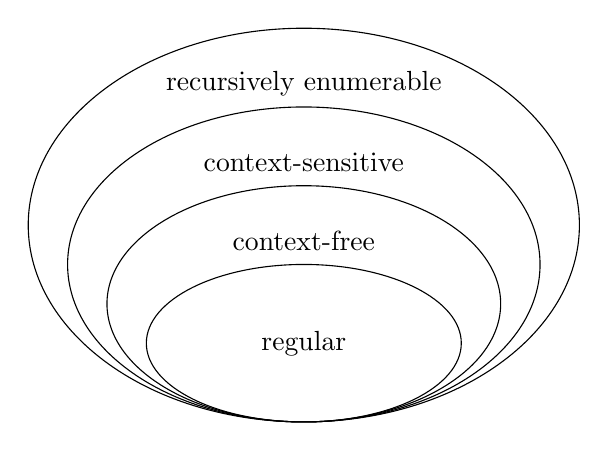
\begin{tikzpicture}
      %TODO: add colours to ellipses without overlapping
      \draw (0,0) ellipse (2 and 1);
      \draw (0,0.5) ellipse (2.5 and 1.5);
      \draw (0,1) ellipse (3 and 2);
      \draw (0,1.5) ellipse (3.5 and 2.5);
      \node at (0,0) {regular};
      \node at (0,1.3) {context-free};
      \node at (0,2.3) {context-sensitive};
      \node at (0,3.3) {recursively enumerable};
  \end{tikzpicture}
  \caption{Chomsky hierarchy of formal languages}
  \label{fig:chomsky-hierarchy}
\end{figure}


Type~3 productions constrain derivations to one non terminal symbol at most,  
ensuring finite memory during parsing.  
The resulting languages coincide with those accepted by finite automata, an insight traced back to Kleene.  

\begin{theorem}[Kleene Correspondence]\label{thm:kleene}
The following families coincide:
\begin{enumerate}
  \item languages generated by type~3 grammars,
  \item languages denoted by regular expressions,
  \item languages recognised by \glspl{cfa}.
\end{enumerate}
\cite{kleene1951representationof}
\end{theorem}

Kleene's theorem supplies three interchangeable viewpoints:  
syntactic derivation, algebraic expression and operational recognition.  
Switching among them allows proofs to borrow the strengths of each representation,  
for instance when optimising a \gls{dfa} derived from a regular expression.  

\begin{proposition}[Closure of \glspl{reg}]\label{prop:closure}
Let ${\cal R}$ denote the class of \glspl{reg}.  
If $L_{1},L_{2}\in{\cal R}$ then so are
$L_{1}\cup L_{2}$, $L_{1}\cap L_{2}$, $\overline{L_{1}}$,
$L_{1}\,L_{2}$ and $L_{1}^{\ast}$ \cite{hopcroft2001introduction}.  
\end{proposition}

Closure under Boolean operations follows directly from set algebra on \gls{dfa} state sets,  
while closure under concatenation and star is established with product and power set constructions.  
These properties justify the pervasive role of \glspl{reg} in software tools:  
complex lexical patterns can be decomposed, manipulated and recombined without leaving ${\cal R}$.  

\begin{theorem}[Myhill-Nerode]\label{thm:myhill-nerode}
A language $L\subseteq\Sigma^{\ast}$ is regular  
iff the relation
$x\equiv_{L}y \;\Longleftrightarrow\; \forall z\in\Sigma^{\ast}\colon  
xz\in L \;\Leftrightarrow\; yz\in L$
admits finitely many equivalence classes \cite{hopcroft2001introduction}.  
\end{theorem}

The theorem supplies a minimality criterion:  
the number of equivalence classes equals the state count of the smallest \gls{dfa} for $L$.  
In compiler construction this bound translates into memory requirements for lexical analysers.  

\begin{example}[Simple \gls{reg}]\label{ex:reg-lang}
For $\Sigma=\{0,1\}$ the set
$L=\{w\in\Sigma^{\ast}\mid w\text{ ends in }1\}$ is regular because it
is described by the regular expression $\Sigma^{\ast}1$ \cite{hopcroft2001introduction}.  
\end{example}

The language of Example~\ref{ex:reg-lang} illustrates how a single positional constraint  
is captured by a two-state \gls{dfa}, matching the Myhill-Nerode bound.  

\begin{observation}\label{obs:why-regular-matters}
\glspl{reg} admit linear time membership tests and deterministic
finite-state representations; therefore they are widely used in lexical
tokenisers, model checking and hardware controllers \cite{aho1974design}.  
\end{observation}

In summary, regularity offers a balance between expressive adequacy for many practical patterns  
and tractable analysis, providing the theoretical bedrock on which later subsections build deterministic,  
nondeterministic and quantum extensions of the finite automaton paradigm.

\subsection{Deterministic Finite Automaton}\label{subsec:dfa}

Among abstract machines the \gls{dfa} offers the most transparent model
of computation.  From any configuration the current state and the symbol
under the input head select exactly one successor state
\cite{hopcroft2001introduction}.  This functional behaviour yields predictable
memory usage, permits direct hardware realisation and supports efficient
software simulation.

\begin{definition}[Deterministic Finite Automaton]\label{def:dfa}
A \gls{dfa} is a quintuple
$M=(Q,\Sigma,\delta,q_{0},F)$ where
$Q$ is a finite set of states,
$\Sigma$ is an input alphabet,
$\delta\colon Q{\times}\Sigma\to Q$ is the transition map,
$q_{0}\in Q$ is the start state and
$F\subseteq Q$ is the set of accepting states
\cite{hopcroft2001introduction}.
\end{definition}

For analysis it is convenient to lift $\delta$ to words.  The extended
map $\hat{\delta}\colon Q{\times}\Sigma^{\ast}\to Q$ satisfies
$\hat{\delta}(q,\varepsilon)=q$ and
$\hat{\delta}(q,aw)=\hat{\delta}(\delta(q,a),w)$.  Structural induction
on the length of $w$ shows that $\hat{\delta}$ is total and unique
\cite{hopcroft2001introduction}.

\begin{proposition}[Unique computation path]\label{prop:dfa-path}
For every input word $w\in\Sigma^{\ast}$ the sequence
$\,q_{0},
\hat{\delta}(q_{0},a_{1}),
\hat{\delta}(q_{0},a_{1}a_{2}),
\dots,
\hat{\delta}(q_{0},w)\,$
is the only path in $M$ labelled by $w$
\cite{hopcroft2001introduction}.
\end{proposition}

\begin{definition}[Accepted language]\label{def:dfa-lang}
The language recognised by $M$ is
$L(M)=\{\,w\in\Sigma^{\ast}\mid \hat{\delta}(q_{0},w)\in F\,\}$
\cite{hopcroft2001introduction}.
\end{definition}

Finite automata gain analytic power from the right invariant congruence
\[x\equiv_{L}y \Longleftrightarrow
  \forall z\in\Sigma^{\ast}\colon
  xz\in L \Leftrightarrow yz\in L.\]

\begin{theorem}[Myhill Nerode]\label{thm:mn-dfa}
A language $L\subseteq\Sigma^{\ast}$ is regular
iff the relation $\equiv_{L}$ has finitely many equivalence classes
\cite{nerode1958linear}.
\end{theorem}

The number of classes equals the size of the smallest \gls{dfa} for $L$,
so state minimisation amounts to quotienting by $\equiv_{L}$.

\begin{theorem}[DFA minimisation]\label{thm:minimisation}
Every \gls{dfa} $M$ possesses a unique minimal
equivalent \gls{dfa} $M_{\mathrm{min}}$ up to isomorphism
\cite{moore1956gedanken}. The Hopcroft partition refinement algorithm computes
$M_{\mathrm{min}}$ in $O(|Q|\log|Q|)$ time \cite{hopcroft1971n}.
\end{theorem}

Because a \gls{dfa} is finite, many questions are decidable.

\begin{proposition}[Algorithmic questions]\label{prop:dfa-decision}
Given \glspl{dfa} $M_{1},M_{2}$ over $\Sigma$ one can decide in
polynomial time: emptiness of $L(M_{1})$, finiteness of $L(M_{1})$,
equivalence $L(M_{1})=L(M_{2})$ and inclusion
$L(M_{1})\subseteq L(M_{2})$ \cite{hopcroft2001introduction}.
\end{proposition}

\begin{example}[Even number of \(a\) symbols]\label{ex:dfa-even}
Figure~\ref{fig:dfa-even-a} depicts the \gls{dfa} recognising
$L=\{\,w\in\{a,b\}^{\ast}\mid
       \text{the number of }a\text{ symbols is even}\,\}$
\cite{hopcroft2001introduction}.  The relation $\equiv_{L}$ has exactly two
classes, matching the two states shown.
\end{example}

\begin{figure}[H]
    \centering
    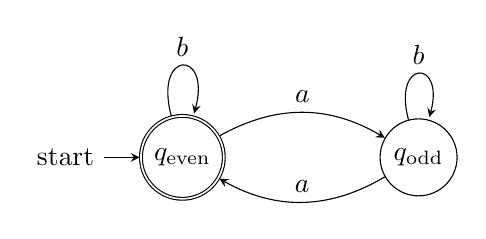
\begin{tikzpicture}[->,>=stealth,node distance=30mm]
      \node[state,initial,accepting] (qe) {$q_{\mathrm{even}}$};
      \node[state]                   (qo) [right of=qe] {$q_{\mathrm{odd}}$};
      \path (qe) edge[loop above] node {$b$} (qe)
            (qo) edge[loop above] node {$b$} (qo)
            (qe) edge[bend left, sloped, above]  node {$a$} (qo)
            (qo) edge[bend left, sloped, above]  node {$a$} (qe);
    \end{tikzpicture}
    \caption{\gls{dfa} for words with an even number of \(a\) symbols
    \cite{hopcroft2001introduction}.}
    \label{fig:dfa-even-a}
\end{figure}

\begin{example}[Binary multiples of three]\label{ex:dfa-mult3}
Over $\Sigma=\{0,1\}$ the set
$L=\{\,w\mid w\text{ interpreted as binary represents a multiple of }3\,\}$
is regular.  A machine with three states tracks the remainder modulo
three after each bit is read \cite{sipser1996introduction}.
\end{example}

\glspl{dfa} support linear time scanning with constant memory.
Compilers use them for lexical analysis, hardware circuits translate
transitions into flip flops, and many regular expression engines adopt
deterministic evaluation to guarantee predictable performance
\cite{aho1974design}.  Deterministic automata thus form the
baseline against which later sections measure the expressive gains and
computational costs of nondeterministic, weighted and quantum variants.

\subsection{Nondeterministic Finite Automaton}\label{subsec:nfa}

Where a \gls{dfa} follows a single computation path, a \gls{nfa} may
branch whenever several successor states are permitted.  The branching
semantics can reduce the number of states that must be stored
explicitly, but it transfers complexity to the acceptance relation
\cite{rabin1959finite}.

\begin{definition}[Nondeterministic Finite Automaton]\label{def:nfa}
A \gls{nfa} is a quintuple
$M=(Q,\Sigma,\delta,q_{0},F)$ with
finite-state set $Q$, input alphabet $\Sigma$, transition map
$\delta\colon Q{\times}\Sigma_{\varepsilon}\to\mathcal{P}(Q)$,
start state $q_{0}\in Q$ and set of final states $F\subseteq Q$.
Here $\Sigma_{\varepsilon}=\Sigma\cup\{\varepsilon\}$ adjoins the empty
word to allow silent moves \cite{rabin1959finite}.
\end{definition}

Extending $\delta$ to words first requires the
$\varepsilon$-closure operator
$\operatorname{E}(S)=
  \bigl\{\,q\in Q\mid
          \exists p\in S\colon
          p\xrightarrow{\varepsilon^{\ast}} q\,\bigr\}$

For $w=a_{1}a_{2}\dots a_{n}$ define recursively  
$S_{0}=\operatorname{E}\bigl(\{q_{0}\}\bigr)$ and  
$S_{i+1}=  
\operatorname{E}\bigl(\,\bigcup_{q\in S_{i}}\delta(q,a_{i+1})\bigr)$.
The set $S_{n}$ collects every state reachable after reading $w$.

\begin{lemma}[Acceptance criterion]\label{lem:nfa-accept}
The automaton $M$ accepts $w$ exactly when
$S_{|w|}\cap F\neq\emptyset$ \cite{hopcroft2001introduction}.
\end{lemma}

Nondeterminism does not enlarge expressive power.

\begin{theorem}[Subset construction]\label{thm:subset}
For an \gls{nfa} with $n$ states the powerset construction produces an
equivalent \gls{dfa} whose state set has size at most $2^{n}$
\cite{rabin1959finite}.  
\end{theorem}

Silent moves can be eliminated first; the combined transformation
preserves language and produces a \gls{dfa} whose transition map
operates on subsets of $Q$.

\begin{proposition}[Elimination of $\varepsilon$ transitions]\label{prop:eps-removal}
An \gls{nfa} with $\varepsilon$ moves has an equivalent
$\varepsilon$-free \gls{nfa} with the same number of states
\cite{hopcroft2001introduction}.
\end{proposition}

Although determinisation may yield an exponential blow-up, the reverse
direction is more benign.

\begin{observation}[Succinctness gap]\label{obs:nfa-size}
There exist languages $L_{n}\subseteq\Sigma^{\ast}$ whose minimal
\gls{nfa} requires $\Theta(n)$ states while every equivalent
\gls{dfa} needs $\Theta(2^{n})$ states
\cite{aho1974design}.
\end{observation}

The gap justifies the preference for \glspl{nfa} as intermediate
representations in regular expression engines that ultimately generate a
\gls{dfa} only for performance critical fragments.

\begin{example}[Words of length one]\label{ex:nfa-length1}
Figure~\ref{fig:nfa-figure} shows a four state \gls{nfa} that accepts
$\Sigma^{1}$.  Two silent moves branch from $q_{0}$; each branch consumes
one symbol then moves to the final state $q_{f}$
\cite{rabin1959finite}.
\end{example}

\begin{figure}[H]
    \centering
    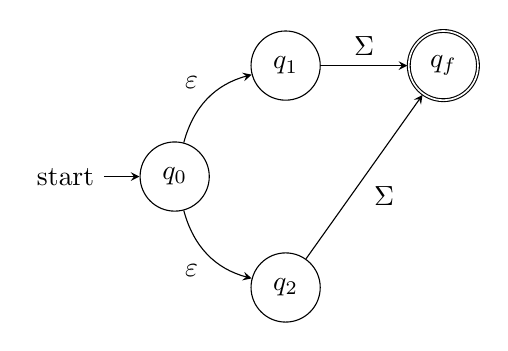
\begin{tikzpicture}[->,>=stealth,node distance=11mm,auto]
      \node[state,initial] (q0) {$q_{0}$};
      \node[state]         (q1) [above right=of q0] {$q_{1}$};
      \node[state]         (q2) [below right=of q0] {$q_{2}$};
      \node[state,accepting] (qf) [right=of q1] {$q_{f}$};
      %
      \path (q0) edge[bend left]  node {$\varepsilon$} (q1)
            (q0) edge[bend right] node[swap] {$\varepsilon$} (q2)
            (q1) edge node {$\Sigma$} (qf)
            (q2) edge node[swap] {$\Sigma$} (qf);
    \end{tikzpicture}
    \caption{\gls{nfa} for all words whose length equals one
             \cite{rabin1959finite}.}
    \label{fig:nfa-figure}
\end{figure}

Decision problems for \glspl{nfa} inherit tractability from their
deterministic counterparts because determinisation is constructive;
emptiness, finiteness and equivalence remain decidable in polynomial
time with respect to the size of the generated \gls{dfa}
\cite{hopcroft2001introduction}.  Subsequent sections compare these classical
results with the complexity landscape of probabilistic and quantum
extensions.

\subsection{Probabilistic Finite Automaton}\label{subsec:pfa}

\glspl{cfa} represent discrete control without any source
of uncertainty.  By attaching probabilities to transitions we obtain a
model that evolves like a Markov chain driven by the scanned word.
These \glspl{pfa} form the finite-memory analogue of probabilistic
Turing machines and supply the algebraic core of hidden Markov models
\cite{rabin1963probabilistic}.

\begin{definition}[Probabilistic Finite Automaton]\label{def:pfa}
  A \gls{pfa} is a quintuple
  \[
    M=(Q,\Sigma,\{\delta(a)\}_{a\in\Sigma},\mathbf{i},F)
  \]
  where
  \begin{itemize}
    \item $Q$ is a finite-state set,
    \item $\Sigma$ is an input alphabet,
    \item for every $a\in\Sigma$ the matrix
          $\delta(a)\in[0,1]^{Q\times Q}$ is
          row-stochastic, that is
          $\sum_{q'\in Q}\delta(a)_{q,q'}=1$ for each $q\in Q$,
    \item $\mathbf{i}\in[0,1]^{Q}$ is a row vector that lists the initial
          state distribution with $\sum_{q\in Q}\mathbf{i}_{q}=1$,
    \item $F\subseteq Q$ is the set of accepting states
          \cite{rabin1963probabilistic}.
  \end{itemize}
\end{definition}
  

Reading a word $w=a_{1}a_{2}\dots a_{n}$ multiplies the matrices that
correspond to its symbols, producing the distribution
\[
  \mathbf{p}(w)=
  \mathbf{i}\,\delta(a_{1})\delta(a_{2})\dots\delta(a_{n}).
\]
The acceptance probability is then
$\Pr_{M}(w)=\sum_{q\in F}\mathbf{p}(w)_{q}$.

\begin{concept}[Cut point language]\label{concept:cutpoint}
For any threshold $\lambda\in[0,1]$ define
\[
  L(M,\lambda)=
  \{\,w\in\Sigma^{\ast}\mid\Pr_{M}(w)>\lambda\,\}
\]
\end{concept}\cite{rabin1963probabilistic}.

Where deterministic and nondeterministic machines yield yes / no
answers, a \gls{pfa} induces a family of cut point languages by varying
$\lambda$.  This observation motivates the notion of stochastic
recognition.

\begin{definition}[Stochastic language]\label{def:stoch}
A language $L\subseteq\Sigma^{\ast}$ is called stochastic if
there exist a \gls{pfa} $M$ and a cut point $\lambda$ such that
$L=L(M,\lambda)$ \cite{rabin1963probabilistic}.  The family of all stochastic
languages is written $\mathsf{SL}$.
\end{definition}

Unlike nondeterminism, randomisation enlarges expressive power.

\begin{theorem}[Non regular stochastic languages]\label{thm:stoch-nonreg}
There exists $L\in\mathsf{SL}\setminus\mathsf{REG}$; consequently
$\mathsf{SL}$ strictly contains the \glspl{reg}
\cite{rabin1963probabilistic}.
\end{theorem}

The price of this extra power is undecidability.

\begin{proposition}[Undecidable properties]\label{prop:pfa-undec}
For unbounded-error \glspl{pfa} the problems of emptiness,
universality and equivalence are undecidable \cite{paz2014introduction}.
\end{proposition}

Bounding the error restores regularity.

\begin{theorem}[Bounded-error regularity]\label{thm:pfa-bounded}
If there exists $\eta>0$ such that
$\lvert\Pr_{M}(w)-\lambda\rvert\ge\eta$ for every
$w\in\Sigma^{\ast}$, then $L(M,\lambda)$ is regular
\cite{paz2014introduction}.
\end{theorem}

Even under bounded error, randomised machines can be exponentially more
succinct than deterministic ones.

\begin{observation}[State complexity]\label{obs:pfa-states}
Some \glspl{reg} admit \glspl{pfa} of $\Theta(n)$ states, whereas
any equivalent \gls{dfa} needs $\Theta(2^{n})$ states
\cite{paz2014introduction}.
\end{observation}

\begin{example}[Unary majority]\label{ex:pfa-majority}
Let $\Sigma=\{a,b\}$ and
\[
  L=\{\,w\in\Sigma^{\ast}\mid\#_{a}(w)>\#_{b}(w)\,\}.
\]
A two-state \gls{pfa} with cut point $\lambda=\tfrac12$ recognises $L$
by interpreting each $a$ as a biased step toward the accepting state and
each $b$ as a step in the opposite direction
\cite{rabin1963probabilistic}.  The pumping lemma shows that $L$ is not regular,
illustrating Theorem~\ref{thm:stoch-nonreg}.
\end{example}

\begin{figure}[H]
    \centering
    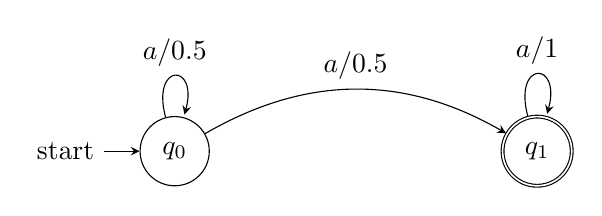
\begin{tikzpicture}[->,>=stealth,node distance=37mm,auto]
      \node[state,initial]   (q0) {$q_{0}$};
      \node[state,accepting] (q1) [right=of q0] {$q_{1}$};
      \path (q0) edge[loop above] node {$a/0.5$} (q0)
            (q0) edge[bend left]  node {$a/0.5$} (q1)
            (q1) edge[loop above] node {$a/1$} (q1);
    \end{tikzpicture}
    \caption{\gls{pfa} that recognises
             $\{a^{k}\mid k\ge2\}$ with cut point $\lambda=0.5$
             \cite{rabin1963probabilistic}.}
    \label{fig:pfa-figure}
\end{figure}

Early stochastic automata not only foreshadowed subsequent models of
probabilistic computation but also laid the groundwork for practical
hidden Markov models in speech and bioinformatics
\cite{rabin1963probabilistic,paz2014introduction}.  Taken together, these results show that
probability enriches finite-state computation while sharply separating
efficient description from decidable analysis, a theme that recurs in
quantum and weighted automata studied in the following sections.

\subsection{Two-Way Variants}\label{subsec:two-way}

Permitting the reading head to move left as well as right
gives \glspl{fa} a bidirectional scanning ability.
This operational freedom simplifies many pattern recognisers
yet, perhaps surprisingly, does not extend expressive power
beyond the \glspl{reg}
\cite{shepherdson1959reduction}.

\begin{definition}[Bidirectional Head]\label{def:two-way-head}
Let $\Sigma_{\Box}=\Sigma\cup\{\Box\}$, where $\Box$ marks the left
end of the input.  A head movement is specified by
$d\in\{-1,0,1\}$, meaning
left, stay, or right
\cite{shepherdson1959reduction}.
\end{definition}

With the motion primitive in place we distinguish three probabilistic
levels of control.

\begin{definition}[2DFA, 2NFA, 2PFA]\label{def:2dfa2nfa2pfa}
A bidirectional automaton is a quintuple
$M=(Q,\Sigma_{\Box},\delta,q_{0},F)$ that differs only
in the type of its transition map $\delta$.
\begin{itemize}
  \item \gls{2dfa}\,:  
        $\delta\colon Q\times\Sigma_{\Box}\to
                   Q\times\{-1,0,1\}$ is a function.
  \item \gls{2nfa}\,:  
        $\delta$ maps to finite sets of
        state-move pairs, introducing nondeterminism
        \cite{rabin1959finite}.
  \item \gls{2pfa}\,:  
        for every symbol $a$
        the distribution
        $\delta(\cdot\mid a)$ is row-stochastic over
        $Q\times\{-1,0,1\}$, yielding a Markov
        decision process
        \cite{freivalds1981probabilistic}.
\end{itemize}
\end{definition}

Bidirectional motion changes how a language is processed rather than
which languages can be processed.

\begin{theorem}[Expressive Power]\label{thm:two-way-reg}
Deterministic, nondeterministic and bounded-error probabilistic
bidirectional automata
recognise exactly the \glspl{reg}
\cite{shepherdson1959reduction,freivalds1981probabilistic}.
\end{theorem}

Although the recognised class is unchanged, determinising a bidirectional
machine can be costly.

\begin{proposition}[Simulation Cost]\label{prop:two-way-cost}
\leavevmode\vspace{-0.5\baselineskip}
\begin{itemize}
  \item An \(n\)\,state \gls{2dfa} or \gls{2nfa} may require
        \(2^{\mathcal{O}(n\log n)}\) states when simulated by a \gls{1dfa}
        \cite{shepherdson1959reduction,rabin1959finite}.
  \item A bounded-error \gls{2pfa} expands to
        $\mathcal{O}(n^{2})$ states under conversion to
        a \gls{1pfa}
        \cite{dwork1992finite}.
\end{itemize}
\end{proposition}

Bidirectional automata therefore occupy an interesting
middle-ground: they match one-way machines in expressive power while
often providing exponentially more succinct descriptions.

\begin{observation}[Practical Motivation]\label{obs:two-way-app}
Repeated passes over data streams are common in text editors,
network-protocol monitors and reversible parsing.
Bidirectional automata give a concise formal model of this behaviour
\cite{shepherdson1959reduction}.
\end{observation}

In summary, allowing the head to retrace its steps enriches algorithmic
strategy and can yield dramatic savings in state count,
yet all such advantages remain confined within the \glspl{reg}
frontier that anchors the theory developed in the previous subsections.

\section{Quantum Mechanics Foundations}
\label{sec:qm-foundations}

Quantum theory delivers a linear-algebraic description of microscopic
systems that has withstood every experimental test to date
\cite{dirac1981principles,nielsen2010quantum}. The finite-dimensional fragment of
this theory already suffices for reversible computing,
cryptography and the automata models investigated later in the thesis.
Accordingly the presentation below restricts attention to finite
Hilbert spaces and the unitary maps that act upon them.

The narrative proceeds from kinematic notions to dynamical ones.
First come pure quantum states, qubits and Dirac's bra-ket notation,
followed by the tensor product that builds composite systems and the
Bloch-sphere picture that aids visualisation of single-qubit
superposition. Entanglement is then introduced as the key non-classical
resource, together with Schmidt rank as a quantitative measure.
Measurement postulates appear next, encompassing both projective
measurements and the more general \glspl{povm} that
model noisy detectors. Density operators, partial trace and quantum
channels provide the language for open-system dynamics, while Kraus
decompositions formalise decoherence and error. Finally the Schrödinger
equation is specialised to finite-dimensional unitary evolution,
establishing the toolkit used in subsequent chapters on quantum finite
automata.

Relativistic extensions handled by quantum field theory, such as those described by the \gls{qft}, remain outside the present scope \cite{weinberg1995quantum}; every
example and proof will rely only on the finite-dimensional machinery
summarised here.

\subsection{Qubits and Quantum States}

Quantum information is encoded in the state of a two-level system, the
\gls{qubit}. Although physical realisations differ, ranging from
photonic polarisations and superconducting circuits to nuclear spins, the mathematical
model is uniform: a unit vector in a two-dimensional complex Hilbert
space \cite{dirac1981principles,nielsen2010quantum}. Dirac's bra-ket notation
offers a compact syntax for such vectors and fixes
\(\{\ket{0},\ket{1}\}\) as the computational basis used
throughout the thesis.

\begin{definition}[Pure qubit state]\label{def:pure-qubit}
A pure state of a qubit is a unit vector
\[
 \ket{\psi}= \alpha\ket{0}+\beta\ket{1},
 \qquad
 \alpha,\beta\in\mathbb C,\;
 |\alpha|^{2}+|\beta|^{2}=1.
\]
Equivalently one may parameterise the state as
\[
 \ket{\psi}=\cos\frac{\theta}{2}\ket{0}
       +e^{\mathrm i\phi}\sin\frac{\theta}{2}\ket{1},
 \qquad
 \theta\in[0,\pi],\;\phi\in[0,2\pi),
\]
where the pair \((\theta,\phi)\) locates \(\ket{\psi}\) on the Bloch
sphere \cite{nielsen2010quantum}.
\end{definition}

The Bloch sphere embeds all pure qubit states on the surface of a unit
sphere in \(\mathbb R^{3}\); its poles represent the basis vectors while
global phases \(e^{\mathrm i\gamma}\ket{\psi}\) collapse to the same
point because overall phase has no observable consequence
\cite{nielsen2010quantum}. Figure~\ref{fig:bloch_sphere} displays the geometry
and the two angular coordinates that parameterise a state.

\begin{figure}[ht]
 \centering
 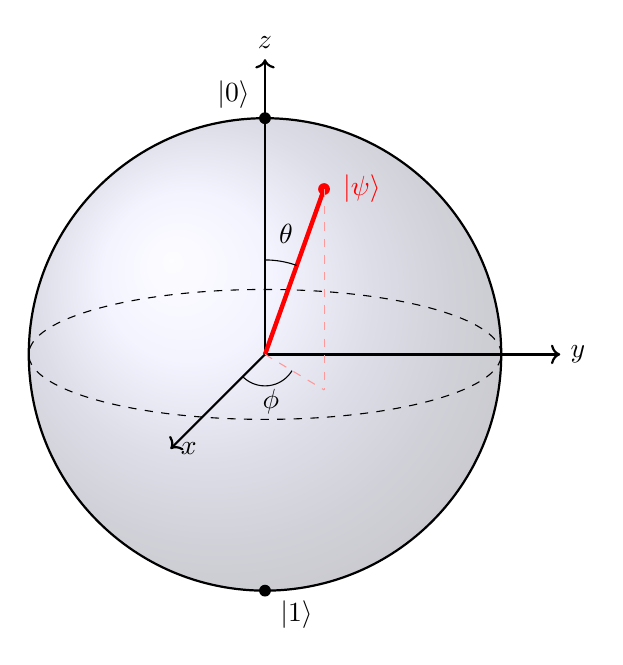
\begin{tikzpicture}[scale=1.5]
  \shade[ball color=blue!20, opacity=0.3] (0,0) circle (2cm);
  \draw[thick] (0,0) circle (2cm);
  \draw[dashed] (0,0) ellipse (2cm and 0.55cm);
  \draw[->, thick] (0,0) -- (2.5,0) node[right] {$y$};
  \draw[->, thick] (0,0) -- (0,2.5) node[above] {$z$};
  \draw[->, thick] (0,0) -- (-0.8,-0.8) node[right] {$x$};
  \fill (0,2) circle (0.05);
  \fill (0,-2) circle (0.05);
  \node[above, xshift=-0.4cm] at (0,2) {\(\ket{0}\)};
  \node[below, xshift=0.4cm] at (0,-2) {\(\ket{1}\)};
  \draw[red, ultra thick] (0,0) -- (0.5,1.4) node[right] {\(\;\ket{\psi}\)};
  \fill[red] (0.5,1.4) circle (0.05);
  \draw[dashed, red!40] (0.5,1.4) -- (0.5,-0.3);
  \draw[dashed, red!40] (0,0) -- (0.5,-0.3);
  \coordinate (O) at (0,0);
  \coordinate (N) at (0,2);
  \coordinate (B) at (0.5,1.4);
  \coordinate (T) at (0.5,-0.3);
  \coordinate (X) at (-0.8,-0.8);
  \pic [shift={(0,0.5)}, draw, "$\theta$", angle eccentricity=1.3, angle radius=1.2cm] {angle = B--O--N};
  \pic [draw, "$\phi$", angle eccentricity=1.5, angle radius=0.4cm] {angle = X--O--T};
 \end{tikzpicture}
 \caption{The Bloch sphere representation of a qubit.}
 \label{fig:bloch_sphere}
 \end{figure}

 Composite systems are modelled by tensor products. Two qubits \(A\) and
 \(B\) inhabit
 \(\mathcal H_{AB}=\mathcal H_{2,A}\otimes\mathcal H_{2,B}\), enabling
 entangled states such as the Bell pair
 \(\ket{\Phi^{+}}=\tfrac{1}{\sqrt2}(\ket{00}+\ket{11})\). Mixed states,
 described by density operators \(\rho\) with
 \(\rho\ge0\) and \(\operatorname{tr}\rho=1\), appear later when noise
 and measurement are introduced; for the purely kinematic discussion
 here, pure vectors suffice.
 
 The qubit therefore serves as the atomic carrier of quantum information,
 combining a continuous state space with a discrete computational basis.
 Subsequent subsections build on this representation, first to formalise
 measurement and decoherence, then to construct \glspl{qfa}
 whose internal registers are composed of a finite number of qubits.

 \subsection{Superposition and Entanglement}\label{subsec:superposition_entanglement}

 Quantum information is encoded in vectors of a finite-dimensional Hilbert space~$\mathcal H$.  
 Linearity of~$\mathcal H$ implies that a linear combination of admissible vectors is again an admissible vector.  
 
 \begin{definition}[Principle of superposition {\cite{nielsen2010quantum}}]
   Let $\{\ket{\psi_i}\}_{i\in I}\subset\mathcal H$ be a family of normalised state vectors and let $\{\alpha_i\}_{i\in I}\subset\mathbb C$ satisfy $\sum_{i\in I}\lvert\alpha_i\rvert^2=1$.  
   The vector $\ket{\Psi}=\sum_{i\in I}\alpha_i\ket{\psi_i}$ is a valid quantum state and is called a superposition of the~$\ket{\psi_i}$.
 \end{definition}
 
 Superposition yields interference phenomena that have no classical counterpart; amplitudes, not probabilities, add.  
 In protocols such as the Deutsch-Jozsa algorithm and amplitude amplification the relative phases between components of~$\ket{\Psi}$ are adjusted in order to concentrate probability mass on measurement outcomes that reveal global properties of the input~\cite{nielsen2010quantum}.  
 
 \begin{remark}
   For a single qubit any pure state can be written as $\ket{\psi}=\cos\frac\theta2\ket{0}+e^{i\phi}\sin\frac\theta2\ket{1}$ with $\theta\in[0,\pi]$ and $\phi\in[0,2\pi)$.  
   This parametrisation maps one-to-one to the Bloch sphere and offers geometric insight into unitary control operations.
 \end{remark}
 
 
 Composing systems is formalised by the tensor product.  
 Let $\mathcal H_A$ and $\mathcal H_B$ be Hilbert spaces for subsystems~$A$ and~$B$.  
 A joint pure state lives in $\mathcal H_{AB}=\mathcal H_A\otimes\mathcal H_B$.  
 Some joint states are separable; others are not.
 
 \begin{definition}[Entangled state {\cite{horodecki2009quantum}}]\label{def:entangled}
   A pure state $\ket{\Psi}_{AB}\in\mathcal H_{AB}$ is entangled if there exist no states $\ket{\psi}_A\in\mathcal H_A$ and $\ket{\phi}_B\in\mathcal H_B$ such that $\ket{\Psi}_{AB}=\ket{\psi}_A\otimes\ket{\phi}_B$.
 \end{definition}
 
 \begin{example}[Bell pair {\cite{bell1964einstein}}]
   The state
   \[
     \ket{\Psi^-}=\frac1{\sqrt2}\bigl(\ket{0}_A\ket{1}_B-\ket{1}_A\ket{0}_B\bigr)
   \]
   is entangled.  
   Tracing out either subsystem produces the maximally mixed single-qubit density operator $\frac12I$, confirming that no local description captures the correlations present in~$\ket{\Psi^-}$.
 \end{example}
 
 \begin{proposition}[Schmidt criterion {\cite{nielsen2010quantum}}]
   A bipartite pure state is separable if and only if its Schmidt rank equals~$1$.
 \end{proposition}
 
 \begin{proof}[Sketch]
   Write $\ket{\Psi}_{AB}=\sum_i\lambda_i\ket{u_i}_A\otimes\ket{v_i}_B$ with orthonormal families $\{\ket{u_i}\}$, $\{\ket{v_i}\}$ and $\lambda_i>0$.  
   If only one Schmidt coefficient is non-zero then $\ket{\Psi}_{AB}$ factorises; conversely, factorisation implies a single non-zero coefficient.  
 \end{proof}
 
 
 Entanglement is a resource underpinning quintessential quantum protocols.  
 It enables perfect teleportation of an unknown qubit state and doubles the classical capacity of a single qubit through superdense coding~\cite{bennett1993teleporting}.  
 Experimentally, violations of Bell inequalities exclude local hidden-variable theories and confirm the non-classical character of entangled correlations~\cite{aspect1982experimental}.  
 
 \begin{remark}
   Entanglement extends beyond two parties.  
   Greenberger-Horne-Zeilinger states and graph states furnish multipartite resources for measurement-based quantum computation.  
   Resource theories quantify entanglement via monotones such as the von~Neumann entropy of the reduced state~\cite{horodecki2009quantum}.
 \end{remark}
 
 Entanglement appears implicitly in later chapters: composite state registers of \glspl{qfa} may evolve into non-separable configurations even when each register individually undergoes unitary dynamics.  
 Understanding superposition and entanglement is therefore prerequisite for analysing interference patterns and acceptance probabilities in \glspl{qfa} models.
 \subsection{Measurement and Probabilistic Outcomes}\label{subsec:measurement_probabilistic}

Measurement translates the abstract formalism of quantum mechanics into experimentally accessible numbers.  
The bridge is supplied by the measurement postulates, stated here for finite-dimensional systems~\cite{von2018mathematical,nielsen2010quantum}.

\begin{definition}[Observable {\cite{von2018mathematical}}]\label{def:observable}
	An observable is a Hermitian operator $M\in\mathcal L(\mathcal H)$ that admits the spectral decomposition
	\[
		M=\sum_{m}m\,\Pi_{m},
	\]
	with orthogonal projectors $\{\Pi_{m}\}$ satisfying $\Pi_{m}\Pi_{m'}=\delta_{m,m'}\Pi_{m}$ and $\sum_{m}\Pi_{m}=\mathbb I$.
\end{definition}

\begin{definition}[Projective measurement \cite{born1925quantentheorie}]\label{def:projective_measurement}
	Let $M$ be an observable with eigenstates $\{\ket{m}\}$ and projectors $\Pi_{m}= \ket{m}\bra{m}$.  
	For an input state $\ket{\psi}$ the probability of obtaining outcome $m$ is
	\[
		P(m)=\braket{\psi|\Pi_{m}|\psi}=|\braket{m}{\psi}|^{2},
	\]
	and the post-measurement state is
	\[
		\ket{\psi}\longmapsto\frac{\Pi_{m}\ket{\psi}}{\sqrt{P(m)}}=\ket{m}.
	\]
\end{definition}

Projective measurements are often too restrictive: realistic detectors have finite resolution, and many protocols require non-orthogonal outcomes.  
The most general measurement allowed by quantum theory is the \gls{povm}, introduced next.

\begin{definition}[\gls{povm} {\cite{kraus1983states,nielsen2010quantum}}]\label{def:povm}
	A set of positive semi-definite operators $\{E_{k}\}\subset\mathcal L(\mathcal H)$ is a \gls{povm} if $\sum_{k}E_{k}=\mathbb I$.  
	For an input state $\ket{\psi}$ the probability of outcome $k$ is
	\[
		P(k)=\bra{\psi}E_{k}\ket{\psi}.
	\]
	There exist operators $\{M_{k}\}$, called Kraus operators, such that $E_{k}=M_{k}^{\dagger}M_{k}$ and $\sum_{k}M_{k}^{\dagger}M_{k}=\mathbb I$.
\end{definition}

\begin{proposition}[State-update rule {\cite{kraus1983states}}]\label{prop:kraus_update}
	When outcome $k$ of a \gls{povm} is observed, the (unnormalised) post-measurement state is
	$M_{k}\ket{\psi},$
	and the normalised state equals $M_{k}\ket{\psi}/\sqrt{P(k)}$.
\end{proposition}

\begin{example}[Computational-basis measurement]\label{ex:computational_basis}
	For a single qubit define $E_{0}=\ket{0}\bra{0}$ and $E_{1}=\ket{1}\bra{1}$.  
	With $\ket{\psi}=\alpha\ket{0}+\beta\ket{1}$, $|\alpha|^{2}+|\beta|^{2}=1$, one finds
	\[
		P(0)=|\alpha|^{2},\qquad P(1)=|\beta|^{2},
	\]
	in agreement with the Born rule; the post-measurement state collapses to the eigenstate corresponding to the observed outcome.
\end{example}


Linearity of quantum dynamics has a profound implication for information processing.

\begin{theorem}[No-cloning {\cite{wootters1982single,dieks1982communication}}]\label{thm:nocloning}
	There exists no unitary operator $U$ and no fixed blank state $\ket{b}$ such that
	\[
		U\bigl(\ket{\psi}\otimes\ket{b}\bigr)=\ket{\psi}\otimes\ket{\psi}
	\]
	holds for every pure state $\ket{\psi}\in\mathcal H$.
\end{theorem}

\begin{proof}[Sketch]
	Assume such a unitary $U$ exists and consider two non-orthogonal states $\ket{\psi}$ and $\ket{\phi}$.  
	Because unitaries preserve inner products,
	\[
		\braket{\psi|\phi}=\bigl(\braket{\psi|\phi}\bigr)^{2},
	\]
	which implies $\braket{\psi|\phi}\in\{0,1\}$.  
	This contradicts the premise that $\ket{\psi}$ and $\ket{\phi}$ are non-orthogonal; thus no perfect cloner exists.
\end{proof}

The impossibility of perfect cloning secures quantum key distribution, forbids noiseless amplification of unknown signals, and motivates approximate or probabilistic cloning strategies analysed in later chapters~\cite{scarani2005quantum}.
\subsection{Decoherence and Open Systems}\label{subsec:decoherence_open}

Isolated dynamics represent an idealisation; every realistic device exchanges energy and information with uncontrolled external degrees of freedom~\cite{breuer2002theory}.  
A quantum description that ignores the environment replaces pure vectors by statistical operators.

\begin{definition}[Density operator {\cite{nielsen2010quantum}}]\label{def:density}
	A density operator on a Hilbert space~$\mathcal H$ is a positive semidefinite matrix $\rho\in\mathcal L(\mathcal H)$ that satisfies $\operatorname{Tr}\rho=1$.  
	It encodes an ensemble $\{p_{i},\ket{\psi_{i}}\}$ through $\rho=\sum_{i}p_{i}\ket{\psi_{i}}\bra{\psi_{i}}$.
\end{definition}

Pure states correspond to projectors $\rho^{2}=\rho$; mixed states satisfy $\rho^{2}\neq\rho$.


Let $\mathcal H_{S}\otimes\mathcal H_{E}$ denote the Hilbert space of a system~$S$ and its environment~$E$.  
If $\ket{\Psi}_{SE}$ evolves unitarily under $U_{SE}$ the reduced state
\[
	\rho_{S}(t)=\operatorname{Tr}_{E}\bigl[\,U_{SE}(t)\,\rho_{SE}(0)\,U_{SE}^{\dagger}(t)\bigr]
\]
is generally mixed and its off-diagonal elements in a preferred basis decay, a phenomenon called decoherence~\cite{zurek2003decoherence,schlosshauer2004decoherence}.  

\begin{definition}[Quantum channel]\label{def:channel}
	A linear map $\mathcal E:\mathcal L(\mathcal H)\to\mathcal L(\mathcal H)$ is a quantum channel if it is completely positive and trace preserving.
\end{definition}

\begin{proposition}[Kraus representation {\cite{kraus1983states}}]\label{prop:kraus}
	Every completely positive and trace preserving map admits operators $\{L_{k}\}$ on~$\mathcal H$ such that
	\[
		\mathcal E(\rho)=\sum_{k}L_{k}\rho L_{k}^{\dagger},
		\qquad
		\sum_{k}L_{k}^{\dagger}L_{k}=\mathbb I .
	\]
\end{proposition}

\begin{example}[Amplitude-damping channel]\label{ex:amplitude_damp}
	For a qubit let $L_{0}=\begin{psmallmatrix}1&0\\0&\sqrt{1-\gamma}\end{psmallmatrix}$ and
	$L_{1}=\begin{psmallmatrix}0&\sqrt{\gamma}\\0&0\end{psmallmatrix}$ with $0\le\gamma\le1$.  
	The map $\mathcal E_{\gamma}(\rho)=L_{0}\rho L_{0}^{\dagger}+L_{1}\rho L_{1}^{\dagger}$ models spontaneous emission at rate~$\gamma$.  
	Diagonal elements remain unchanged whereas the coherence term $\rho_{01}$ decays as $\rho_{01}\mapsto\sqrt{1-\gamma}\,\rho_{01}$, illustrating decoherence.
\end{example}


When environmental correlations relax quickly (Markovian limit) the family $\{\rho(t)\}_{t\ge0}$ forms a quantum dynamical semigroup with generator in \gls{gksl} form~\cite{gorini1976completely,lindblad1976generators}:

\begin{definition}[Lindblad master equation]\label{def:lindblad}
	For a system Hamiltonian $H$ and Lindblad operators $\{L_{k}\}$ the Markovian evolution obeys
	\[
		\frac{\mathrm d\rho}{\mathrm dt}= -\frac{\mathrm i}{\hbar}[H,\rho]
		+\sum_{k}\Bigl(L_{k}\rho L_{k}^{\dagger}-\tfrac12\{L_{k}^{\dagger}L_{k},\rho\}\Bigr).
	\]
\end{definition}

The generator guarantees complete positivity of the channel $e^{t\mathcal L}$ for all $t\ge0$ and will serve in later chapters to model noise acting on the internal registers of \glspl{qfa}.

\subsection{Unitary Evolution and Quantum Dynamics}\label{subsec:unitary_dynamics}

In the absence of measurements and uncontrollable perturbations, a quantum system is considered closed.
Its state vector evolves according to the postulate of unitary time development~\cite{nielsen2010quantum}.

\begin{definition}[Unitary operator]\label{def:unitary}
	A linear map $U:\mathcal H\longrightarrow\mathcal H$ is unitary if $U^{\dagger}U=UU^{\dagger}=\mathbb I$.  
	Unitary operators form a group under composition and preserve inner products:
	$\braket{\psi|\phi}= \braket{U\psi|U\phi}$ for all $\ket{\psi},\ket{\phi}\in\mathcal H$.
\end{definition}


Dynamics are generated by the system Hamiltonian~$H=H^{\dagger}$ through the time-dependent Schrödinger equation~\cite{schrodingjsr19262}
\[
	\mathrm i\hbar\frac{\mathrm d}{\mathrm dt}\ket{\psi(t)} = H(t)\ket{\psi(t)} .
\]

\begin{proposition}[Propagator]\label{prop:propagator}
	The formal solution is
	\[
		\ket{\psi(t)} = U(t,t_{0})\ket{\psi(t_{0})},
		\qquad
		U(t,t_{0}) = \mathcal T
		\exp\Bigl[-\frac{\mathrm i}{\hbar}\int_{t_{0}}^{t}H(t')\,\mathrm dt'\Bigr],
	\]
	where $\mathcal T$ denotes the time-ordering operator~\cite{nielsen2010quantum}.  
	The propagator satisfies $U(t,t)=\mathbb I$ and the composition law $U(t_{2},t_{0})=U(t_{2},t_{1})U(t_{1},t_{0})$.
\end{proposition}

\begin{remark}[Time independent Hamiltonian]
	If $H$ is constant one has the closed expression
	\[
		U(t,t_{0}) = \exp\bigl[-\mathrm iH(t-t_{0})/\hbar\bigr] ,
	\]
	which implements a one-parameter unitary group generated by $H$~\cite{nielsen2010quantum}.
\end{remark}

\begin{example}[Qubit rotation about the $z$ axis]\label{ex:qubit_rotation}
	For a single qubit let $H=\tfrac{\hbar\omega}{2}\sigma_{z}$.  
	The evolution operator equals
	\[
		U(t,0)=\exp\bigl[-\mathrm i\omega t\,\sigma_{z}/2\bigr]
		=\begin{psmallmatrix}
			 e^{-\mathrm i\omega t/2} & 0 \\[2pt]
			 0 & e^{\mathrm i\omega t/2}
		  \end{psmallmatrix},
	\]
	which produces a phase rotation of the computational basis and leaves probabilities invariant.
\end{example}


Unitary dynamics conserve superposition amplitudes and entanglement resources.  
Non unitary modifications originate from coupling to external degrees of freedom or from measurements, modelled in the preceding subsections.  
A rigorous understanding of unitary time development is essential for analysing quantum algorithms, control protocols and the acceptance dynamics of quantum automata.

\section{Quantum Gates and Circuits}
\label{sec:quantum-gates-and-circuits}

The gate model formulates quantum computation as a sequence of reversible transformations that act on an ordered register of qubits. Each elementary transformation, or quantum logic gate, is represented by a unitary matrix that preserves the norm of the wavefunction and therefore the probabilistic interpretation of quantum states \cite{NCFlips}. By composing gates drawn from a finite universal set such as \gls{hadamard},  \gls{phase}, and \gls{cnot}, any unitary operator on a finite dimensional Hilbert space can be approximated to arbitrary accuracy, providing the foundation on which quantum algorithms like Shor's factoring routine and the \gls{qft} are constructed \cite{Barenco1995elementary,Shor1994}.

Beyond abstract universality, physical realisations impose architectural constraints that influence gate granularity, qubit connectivity, and measurement timing. The criteria articulated by DiVincenzo identify coherent state preparation, high fidelity single and two qubit gates, and reliable read-out as indispensable requirements for scalable devices \cite{divincenzo2000criteria}. Present \gls{nisq} processors satisfy these conditions only approximately, which motivates depth-aware decompositions, noise-adaptive compilation, and the explicit accounting of ancillary resources \cite{Preskill2018nisq}. 

In the context of this thesis, quantum circuits serve as the executable target for the compilation of \glspl{qfa}. Each transition operator of an automaton is mapped to a concrete gate sequence, and every accepting projector is realised by a register measurement that interfaces classical control with coherent evolution. The remainder of this section surveys the primitive gate library, canonical circuit families, and decomposition techniques that together supply the hardware-agnostic substrate on which the automata-to-circuit translation of Chapter~\ref{chap:automata-to-circuits} is built.

\subsection{Common Quantum Gates}
\label{sec:common-quantum-gates}

Quantum logic gates are unitary operators acting on one or more qubits.  
They constitute the elementary instruction set of the gate model of quantum computation \cite{NielsenChuang2010}.  
A single-qubit gate realises a rotation of the Bloch vector, whereas a multi-qubit gate can generate entanglement, an intrinsically non-classical resource \cite{Barenco1995elementary}.  
This subsection recalls the canonical gate library, presents the corresponding matrices, and illustrates their circuit symbols \cite{Koch2022quantikz}.

\subsubsection*{Single-qubit gates: Pauli \(X\), \(Y\), \(Z\)}

The Pauli gates \(X\), \(Y\), and \(Z\) implement rotations by \(\pi\) about the \(x\), \(y\), and \(z\) axes of the Bloch sphere, respectively \cite{NielsenChuang2010}.  
In the computational basis \(\{\ket{0},\ket{1}\}\) they take the forms
\[
X=\begin{pmatrix}0&1\\[2pt]1&0\end{pmatrix},
\qquad
Y=\begin{pmatrix}0&-i\\[2pt]i&0\end{pmatrix},
\qquad
Z=\begin{pmatrix}1&0\\[2pt]0&-1\end{pmatrix}.
\]
The gate \(X\) exchanges the computational basis states and therefore plays the role of a quantum NOT \cite{NCFlips}.  
The gate \(Z\) leaves \(\ket{0}\) invariant while mapping \(\ket{1}\) to \(-\ket{1}\); it is consequently referred to as a phase flip \cite{PhaseFlip}.  
The gate \(Y\) combines a bit flip with an intrinsic phase: \(Y\ket{0} = i\ket{1}\) and \(Y\ket{1} = -\,i\ket{0}\) \cite{NCFlips}.  
All three operators square to the identity (up to a global phase) and mutually anticommute, properties that underpin stabiliser-based error-correction protocols \cite{Gottesman1997stabilizer}.

\begin{figure}[ht]
  \centering
  \begin{quantikz}
    \lstick{$\ket{q}$} & \gate{\mathsf{X}} & \qw
  \end{quantikz}
  \caption{Circuit symbol for the Pauli \(X\) gate.  Replacing the label by \(\mathsf{Y}\) or \(\mathsf{Z}\) yields the symbols for the remaining Pauli rotations.}
  \label{fig:x-gate}
\end{figure}

\subsubsection*{\glsentrylong{hadamard}}
The \gls{hadamard} gate realises a rotation by \(\tfrac{\pi}{2}\) about the axis \((x+z)/\sqrt{2}\) on the Bloch sphere \cite{Deutsch1985}.  Its unitary matrix in the computational basis is
\[
\gls{hadamard}= \frac{1}{\sqrt{2}}
\begin{pmatrix}
1 & 1\\[2pt]
1 & -1
\end{pmatrix}.
\]
Acting on the basis states it produces the equal-weight superpositions
\(\gls{hadamard}\ket{0}= \ket{+}\) and
\(\gls{hadamard}\ket{1}= \ket{-}\), where  
\(\ket{\pm}= (\ket{0}\pm\ket{1})/\sqrt{2}\) define the Hadamard basis \cite{NielsenChuang2010}.  
A second application reverses the transformation since \(\gls{hadamard}^{2}=I\) up to global phase \cite{HadamardIteration}.  
Geometrically, the operation transfers quantum states between the \(Z\) and \(X\) axes of the Bloch sphere, sending \(\ket{0}\) and \(\ket{1}\) to the equator and vice versa \cite{Gibney2019bloch}.  
Because it satisfies \(\gls{hadamard} Z \gls{hadamard}=X\) and \(\gls{hadamard} X \gls{hadamard}=Z\), the gate exchanges the roles of bit-flip and phase-flip operators and is therefore indispensable for basis changes and interference patterns in algorithms such as Deutsch-Jozsa and Grover search \cite{Deutsch1992rapid,Grover1997fast,NCFlips}.

\begin{figure}[ht]
  \centering
  \begin{quantikz}
    \lstick{$\ket{q}$} & \gate{H} & \qw
  \end{quantikz}
  \caption{Circuit symbol for the \gls{hadamard} gate \cite{Koch2022quantikz}.}
  \label{fig:h-gate}
\end{figure}

\subsubsection*{Phase rotations: \gls{phase}, \gls{tgate} and continuous \(R_{z}\)}

Phase rotations apply a relative phase to the state $\ket{1}$ while leaving $\ket{0}$ unchanged \cite{Gottesman1997stabilizer}.  
The \gls{phase} gate introduces a phase of \(\pi/2\) and the \gls{tgate} gate a phase of \(\pi/4\); their unitaries are
\[
\gls{phase}= 
\begin{pmatrix}
1 & 0\\[4pt]
0 & i
\end{pmatrix},
\qquad
\gls{tgate}= 
\begin{pmatrix}
1 & 0\\[4pt]
0 & e^{i\pi/4}
\end{pmatrix},
\]
so that
\(\gls{phase}\ket{1}=i\ket{1}\) and \(\gls{tgate}\ket{1}=e^{i\pi/4}\ket{1}\) \cite{NCFlips}.  
Because \(\gls{phase}^{2}=Z\) and \(\gls{tgate}^{4}=Z\), the operations may be viewed as fractional powers of the Pauli \(Z\) rotation \cite{Bravyi2012magic}.  

Neither gate is involutory; instead their adjoints are
\[
  \gls{phase}^{\dagger} =
  \begin{pmatrix}
    1 & 0\\[4pt]
    0 & -i
  \end{pmatrix},
  \qquad
  \gls{tgate}^{\dagger} =
  \begin{pmatrix}
    1 & 0\\[4pt]
    0 & e^{-i\pi/4}
  \end{pmatrix}.
\]

The discrete set \(\{\gls{hadamard},\gls{phase},\mathrm{CNOT}\}\) generates the Clifford group, which is not universal for quantum computation, but adjoining the non-Clifford \gls{tgate} yields a universal gate library capable of approximating any single-qubit unitary to arbitrary precision \cite{Bravyi2012magic,Dawson2005solovay}.  
In fault-tolerant architectures the cost of magic-state distillation makes the \gls{tgate} the dominant resource, so circuit depth is often quantified by its \(T\)-count \cite{Eastin2013thesis}.

\begin{figure}[ht]
  \centering
  \begin{quantikz}
    \lstick{$\ket{q}$} & \gate{S} & \gate{T} & \qw
  \end{quantikz}
  \caption{Sequential application of an \gls{phase} gate followed by a \gls{tgate}.}
  \label{fig:st-sequence}
\end{figure}

More generally, a rotation about a Pauli axis \(\sigma_{\alpha}\in\{X,Y,Z\}\) through an angle \(\theta\) is
\[
R_{\alpha}(\theta)=\exp\bigl(-i\tfrac{\theta}{2}\sigma_{\alpha}\bigr),
\]
with explicit examples
\[
R_{x}(\theta)=
\begin{pmatrix}
\cos\bigl(\tfrac{\theta}{2}\bigr) & -i\sin\bigl(\tfrac{\theta}{2}\bigr)\\[4pt]
-i\sin\bigl(\tfrac{\theta}{2}\bigr) & \cos\bigl(\tfrac{\theta}{2}\bigr)
\end{pmatrix},
\qquad
R_{z}(\theta)=
\begin{pmatrix}
e^{-i\theta/2} & 0\\[4pt]
0 & e^{i\theta/2}
\end{pmatrix}.
\]
The parameterised family \(\{R_{y}(\theta), R_{z}(\phi)\}\) forms a convenient basis for variational circuits, and any single-qubit unitary admits the Euler decomposition  
\(U=R_{z}(\lambda)\,R_{y}(\theta)\,R_{z}(\phi)\) up to global phase \cite{NielsenChuang2010,Kandala2017hardware}.  
Specialising \(\theta=0,\phi=\pi/2\) or \(\pi/4\) recovers the \gls{phase} and \gls{tgate} operations, respectively.

\subsubsection*{Multi-qubit gates: entangling operations}

Operations acting on two or more qubits can create quantum correlations that admit no classical description \cite{Bell1964}.  
Together with arbitrary single-qubit rotations they supply universality for quantum computation \cite{Barenco1995elementary}.

\subsubsection*{\glsentrylong{cnot}}

The \gls{cnot} gate flips the target qubit conditioned on the control being in the state $\ket{1}$ \cite{NielsenChuang2010}.  
In the ordered basis \{$\ket{00}$,$\ket{01}$,$\ket{10}$,$\ket{11}$\} its unitary is
\[
\gls{cnot}=
\begin{pmatrix}
1&0&0&0\\[4pt]
0&1&0&0\\[4pt]
0&0&0&1\\[4pt]
0&0&1&0
\end{pmatrix},
\]
implementing the map \(\ket{a,b}\mapsto\ket{a,a\oplus b}\).  
Applied to a superposition it generates entanglement, for example
\[
\bigl(\tfrac{\ket{0}+\ket{1}}{\sqrt{2}}\bigr)\!\otimes\!\ket{0}
\xrightarrow{\gls{cnot}}
\tfrac{\ket{00}+\ket{11}}{\sqrt{2}},
\]
a Bell state \cite{Bell1964}.  
\gls{cnot} is self-inverse and belongs to the Clifford group \cite{Gottesman1997stabilizer}.

\begin{figure}[ht]
  \centering
  \begin{quantikz}
    \lstick{$\ket{c}$} & \ctrl{1} & \qw \\
    \lstick{$\ket{t}$} & \targ{} & \qw
  \end{quantikz}
  \caption{Circuit symbol for the \gls{cnot} gate with control \(\ket{c}\) and target \(\ket{t}\) \cite{Koch2022quantikz}.}
  \label{fig:cnot-gate}
\end{figure}

\subsubsection*{\glsentrylong{cz}}

The \gls{cz} gate applies a phase flip to the joint state $\ket{11}$; its matrix is
\[
\gls{cz}=
\begin{pmatrix}
1&0&0&0\\[4pt]
0&1&0&0\\[4pt]
0&0&1&0\\[4pt]
0&0&0&-1
\end{pmatrix}
\]
\cite{NielsenChuang2010}.
It is related to \gls{cnot} by a Hadamard conjugation on the target,
\(\gls{cz}_{(c,t)}=\gls{hadamard}_{t}\,\gls{cnot}_{(c,t)}\,\gls{hadamard}_{t}\) \cite{Barenco1995elementary},  
and arises natively in several hardware platforms where controlled phase interactions dominate \cite{Arute2019supremacy}.

\subsubsection*{\glsentrylong{swap}}

The \gls{swap} gate exchanges the states of two qubits: \(\ket{a,b}\mapsto\ket{b,a}\).  
It decomposes into three \gls{cnot} gates,
\(
\gls{swap}_{(1,2)}=
\gls{cnot}_{1,2}\,
\gls{cnot}_{2,1}\,
\gls{cnot}_{1,2}
\) \cite{Barenco1995elementary}.  
Symbolically it is drawn as two crossing lines with \(\times\) markers on the intersection \cite{Koch2022quantikz}.

\subsubsection*{\glsentrylong{toffoli} and \glsentrylong{cswap} gates}

The three-qubit \gls{toffoli} gate flips a target conditioned on two controls being in $\ket{1}$.  
It is universal for reversible classical computation \cite{Bennett1973logical} and admits a fault-tolerant decomposition using six \glspl{cnot}, seven \glspl{tgate} and single-qubit \gls{hadamard} gates \cite{Amy2013tcount}.  

\begin{figure}[ht]
  \centering
  \begin{quantikz}
    \lstick{$\ket{c_1}$} & \ctrl{2} & \qw \\
    \lstick{$\ket{c_2}$} & \ctrl{1} & \qw \\
    \lstick{$\ket{t}$}   & \targ{} & \qw
  \end{quantikz}
  \caption{Symbol for the \gls{toffoli} gate \cite{Koch2022quantikz}.}
  \label{fig:toffoli}
\end{figure}

The \gls{cswap} gate swaps two targets conditioned on a single control and can be synthesised from \glspl{toffoli} \cite{FredkinGate1982}.  

\subsubsection*{Universality}

Any multi-qubit unitary can be approximated using single-qubit rotations together with \gls{cnot} or \gls{cz} gates \cite{Barenco1995elementary}.  
Consequently sets such as \(\{\gls{hadamard},\gls{tgate},\gls{cnot}\}\) support universal quantum computation, and high-level gates are routinely compiled into the \(R_{z}/R_{x}\)+\gls{cnot} primitives of hardware back-ends like IBM’s \(U_{3}\)+\gls{cnot} basis \cite{Cross2017ibm,fedoriaka2025decomposition}.

\subsection{Types of Quantum Circuits}

Just as one can categorize classical circuits (combinational, sequential, etc.), we can distinguish various types of quantum circuits by their structure and purpose.\cite{NielsenChuang2010} Here we survey several important categories, each illustrated by a simple diagram:

\subsubsection*{Single-Qubit Circuits}

A \textbf{single-qubit circuit} operates on a single qubit (or on multiple qubits but without entangling them).\cite{NielsenChuang2010} It consists of one or more single-qubit gates in sequence.\cite{Barenco1995elementary} Such circuits are conceptually the simplest, effecting arbitrary rotations on a single qubit's state.\cite{NielsenChuang2010} While a single qubit cannot exhibit entanglement, single-qubit subcircuits appear as components of larger algorithms (for example, state preparation or individual qubit rotations in a variational ansatz).\cite{Kandala2017hardware}

An example single-qubit circuit is shown below, taking an initial state $\ket{0}$ and applying a sequence of rotations ($H$, then $T$, then $X$), followed by a measurement:

\begin{quantikz}
\lstick{$\ket{0}$} & \gate{H} & \gate{T} & \gate{X} & \meter{} & \cw \\
\end{quantikz}

\noindent This circuit prepares the state $XTH\ket{0}$ and measures it (the outcome is a probabilistic function of the applied gates).\cite{NielsenChuang2010} In general, any single-qubit unitary can be implemented by an appropriate sequence of $H$, $S$, $T$ (or other rotation) gates, as discussed above.\cite{Dawson2005solovay} Single-qubit circuits are often used to calibrate hardware or illustrate basic quantum phenomena like Bloch-sphere rotations.\cite{Barends2014superconducting}

\subsubsection*{Multi-Qubit Circuits}

A \textbf{multi-qubit circuit} involves two or more qubits with gates that act on multiple qubits (such as CNOT or other entangling gates).\cite{Barenco1995elementary} These circuits can generate entanglement and are necessary for computational tasks where qubit interactions are required.\cite{Bell1964} Multi-qubit circuits range from small entangling subroutines (like creating a Bell pair) to large circuits comprising many interacting gates.\cite{NielsenChuang2010}

As a basic example, consider a two-qubit circuit that creates a Bell state.\cite{Bell1964} Starting from $\ket{00}$, we apply a Hadamard on the first qubit and then a CNOT with the first qubit as control and second as target:

\begin{quantikz}
\lstick{$\ket{0}$} & \gate{H} & \ctrl{1} & \qw \\
\lstick{$\ket{0}$} & \qw   & \targ{} & \qw
\end{quantikz}

\noindent After these gates, the qubits are in the entangled state $\frac{1}{\sqrt{2}}(\ket{00} + \ket{11})$, one of the four Bell states.\cite{Bell1964} In general, multi-qubit circuits may involve many entangling gates.\cite{Arute2019supremacy} For instance, quantum adders, error-correcting code circuits, or oracle circuits for algorithms all involve networks of CNOTs (and related gates) spread across multiple qubits.\cite{Gottesman1997stabilizer} Multi-qubit circuits are the backbone of quantum algorithms, as they carry out the entangling operations that give quantum computing its power.\cite{Shor1994}

\subsubsection*{Parameterized (Variational) Circuits}

A \textbf{parameterized quantum circuit} (PQC) is a circuit that contains gates with continuous parameters (angles) which can be adjusted.\cite{Peruzzo2014vqe} These circuits are central to many \emph{variational quantum algorithms} and quantum machine-learning models.\cite{Cerezo2021variational} By treating gate angles as tunable parameters, one can use a classical optimization loop to iteratively adjust these parameters and minimize a cost function evaluated via quantum measurements.\cite{Peruzzo2014vqe} Such circuits are also called \emph{variational circuits} or \emph{ansatz circuits}.\cite{Kandala2017hardware}

Parameterized circuits often have a regular structure, e.g.\ layers of single-qubit rotations and entangling gates.\cite{Kandala2017hardware} An example 2-qubit parameterized circuit (one layer of a common variational ansatz) is shown below:

\begin{quantikz}
\lstick{$\ket{0}$} & \gate{R_y(\theta_1)} & \ctrl{1} & \gate{R_z(\phi_1)} & \qw \\
\lstick{$\ket{0}$} & \gate{R_y(\theta_2)} & \targ{} & \gate{R_z(\phi_2)} & \qw
\end{quantikz}

\noindent Here each qubit is rotated by some angle $\theta_i$ about $Y$ and then entangled, followed by $Z$-rotations by $\phi_i$. The angles ${\theta_i,\phi_i}$ are free parameters that can be optimized.\cite{Peruzzo2014vqe} Stacking multiple such layers increases the expressive power of the ansatz at the cost of more parameters.\cite{Sim2019expressibility} Variational circuits are used in algorithms like the Variational Quantum Eigensolver (for ground-state energies) and QAOA (Quantum Approximate Optimization Algorithm), as well as in quantum classifiers and neural networks.\cite{Farhi2014qaoa} They exemplify a hybrid quantum-classical approach: the quantum circuit provides a parameterized function, and a classical routine tunes the parameters.\cite{Cerezo2021variational}

\subsubsection*{Measurement-Based Circuits}

A \textbf{measurement-based quantum circuit} refers to a model of quantum computation (the one-way quantum computer) where computation is driven by measurements on an entangled resource state.\cite{Raussendorf2001oneway} One first prepares a large entangled state (typically a \emph{cluster state}) and then performs a sequence of single-qubit measurements.\cite{Briegel2009measurement} The measurement bases and any feed-forward adjustments can implement an arbitrary quantum computation, despite using only measurements during the “computing” phase.\cite{Raussendorf2003measurement}

For example, consider a simple three-qubit linear cluster state.\cite{Raussendorf2001oneway} We start with three qubits in $\ket{+}$ states, entangle neighbors via CZ gates, then measure qubits 1 and 2 while qubit 3 remains unmeasured:

\begin{quantikz}
\lstick{$\ket{+}$} & \ctrl{1} & \qw   & \meter{} & \cw \\
\lstick{$\ket{+}$} & \targ{} & \ctrl{1} & \meter{} & \cw \\
\lstick{$\ket{+}$} & \qw   & \targ{} & \qw
\end{quantikz}

\noindent Depending on the measurement outcomes, the state of qubit 3 corresponds to the result of a quantum computation; conditional $X$ or $Z$ corrections (feed-forward) may be applied.\cite{Raussendorf2003measurement} This model is equivalent in power to the standard gate model—any gate circuit can be translated to a measurement pattern on a cluster state.\cite{Briegel2009measurement}

\subsubsection*{Hybrid Quantum-Classical Circuits}

In the current \gls{nisq} era, many practical algorithms use a \textbf{hybrid quantum-classical} approach, wherein quantum circuits are interleaved with classical processing.\cite{Preskill2018nisq} Variational circuits described above are a prime example: the quantum processor prepares a state and performs measurements, and a classical computer processes those results to adjust parameters for the next round.\cite{Cerezo2021variational} Another example is quantum error correction with feedback, where measurement outcomes (syndrome bits) are fed to classical logic that decides further quantum operations in real-time.\cite{Kelly2015error}

Hybrid circuits leverage the strengths of both paradigms: quantum circuits for state preparation and interference on exponentially large state spaces, and classical computations for flexible control and optimization.\cite{Preskill2018nisq} 

\noindent In this flow, the quantum circuit is executed and measured to evaluate a cost function, and a classical optimizer computes new parameters for the next quantum run.\cite{Cerezo2021variational} Hybrid circuits thus are not a single static circuit but a sequence of partial circuits and classical computations.\cite{Preskill2018nisq} Nonetheless, one can represent a single iteration in an expanded quantum circuit diagram by explicitly including measurement operations mid-circuit and classically-controlled gates.\cite{Kelly2015error}

In summary, the above categories illustrate the diversity of quantum circuit styles. A given quantum algorithm may encompass several of these aspects.\cite{Shor1994} Understanding the circuit types helps in designing and optimizing quantum algorithms for real hardware.\cite{Arute2019supremacy}


\subsection{Example Quantum Algorithms as Circuits}

To see these gates and circuit paradigms in action, we now examine three foundational quantum algorithms and their circuit implementations: the Deutsch-Jozsa algorithm, Grover's search algorithm, and the Quantum Fourier Transform.\cite{NielsenChuang2010} For each, we describe the circuit and how the algorithm leverages quantum gates to achieve a speed-up or functionality beyond classical means.\cite{Preskill2018nisq}

\subsubsection*{Deutsch-Jozsa Algorithm}

The Deutsch-Jozsa (DJ) algorithm is one of the first examples of a quantum algorithm that outperforms the classical deterministic result for a specific problem.\cite{Deutsch1992rapid} The task is to determine whether a Boolean function $f:\{0,1\}^n \to \{0,1\}$ is constant or \emph{balanced}, promised that $f$ is one or the other.\cite{Deutsch1992rapid} Classically, in the worst case $2^{n-1}+1$ queries are required.\cite{Cleve1998dj} The Deutsch-Jozsa quantum algorithm solves it with a single query to an oracle $U_f$ that implements $f$.\cite{Deutsch1992rapid}

The circuit for the Deutsch-Jozsa algorithm is as follows.\cite{NielsenChuang2010} We have $n$ qubits for the input (initialized to $\ket{0\cdots0}$) and one output qubit (initialized to $\ket{1}$). First, a layer of Hadamard gates is applied to all qubits, creating a uniform superposition and putting the output qubit in $\ket{-}$.\cite{Deutsch1992rapid} Next, the oracle $U_f$ is applied, mapping $\ket{x}\ket{y}\to\ket{x}\ket{y\oplus f(x)}$.\cite{Cleve1998dj} Finally, another Hadamard layer is applied to the $n$ input qubits, and they are measured.\cite{NielsenChuang2010}

The complete circuit for $n=2$ is:

\begin{quantikz}
\lstick{$\ket{0}_{q_0}$} & \gate{H} & \gate[3,nwires=2]{U_f} & \gate{H} & \meter{} & \cw \\
\lstick{$\ket{0}_{q_1}$} & \gate{H} &                & \gate{H} & \meter{} & \cw \\
\lstick{$\ket{1}_{q_2}$} & \gate{H} &                & \qw   & \qw   &
\end{quantikz}

In this diagram, $U_f$ is a multi-qubit oracle acting on all three qubits.\cite{Cleve1998dj} The output qubit $q_2$ returns to $\ket{-}$ regardless of $f$, so it is ignored in the final measurement.\cite{NielsenChuang2010} Measuring the input qubits yields $0^n$ if $f$ is constant and a non-zero string if $f$ is balanced.\cite{Deutsch1992rapid}

This works because $U_f$ imprints $(-1)^{f(x)}$ as a phase on the input register (phase kickback).\cite{Cleve1998dj} The final Hadamards perform interference: identical phases yield constructive interference on $\ket{0\cdots0}$, while balanced phases cancel there and appear elsewhere, distinguishing the two cases with certainty in one query.\cite{NielsenChuang2010} The DJ algorithm illustrates how superposition and interference evaluate a global property of a function efficiently.\cite{Deutsch1992rapid}

\subsubsection*{Grover's Search Algorithm}

Grover's algorithm searches an unstructured list of $N=2^n$ items for a marked item, achieving a quadratic speed-up over classical search.\cite{Grover1997fast} Classically one needs $O(N)$ queries; Grover requires $O(\sqrt{N})$.\cite{Boyer1998tight} The algorithm iteratively applies the Grover operator $G = D\,U_f$, where $U_f$ flips the phase of the marked state and $D$ (diffusion) inverts amplitudes about the average.\cite{Brassard2002amplification}

A Grover iteration on $n$ qubits is:

\begin{quantikz}
 \lstick{$\ket{0}^{\otimes n}$}
   & \gate{H^{\otimes n}}
   & \gate{U_f}
   & \gate{D}
   & \meter{} \qwbundle{n}
\end{quantikz}


For $n=2$, marking $\ket{11}$ as the solution, an explicit circuit is:

\begin{quantikz}
\lstick{$\ket{0}$} & \gate{H} & \ctrl{1} & \gate{H} & \gate{X} & \ctrl{1} & \gate{X} & \gate{H} & \meter{} & \cw \\
\lstick{$\ket{0}$} & \gate{H} & \gate{Z} & \gate{H} & \gate{X} & \targ{} & \gate{X} & \gate{H} & \meter{} & \cw
\end{quantikz}

Here the first Hadamards create a uniform superposition.\cite{Grover1997fast} The oracle $U_f$ is the controlled-$Z$ on $\ket{11}$.\cite{Brassard2002amplification} The remaining gates implement diffusion: $H^{\otimes n}X^{\otimes n}Z_{\ket{0^n}}X^{\otimes n}H^{\otimes n}$.\cite{NielsenChuang2010} Repeating $r\approx\frac{\pi}{4}\sqrt{N}$ iterations maximizes success probability.\cite{Grover1997fast,Boyer1998tight} Grover thus exploits amplitude amplification to boost the marked state's probability quadratically faster than classical search.\cite{Brassard2002amplification}


\subsubsection*{Quantum Fourier Transform (QFT)}

The Quantum Fourier Transform is a quantum analogue of the discrete Fourier transform applied to the amplitudes of a quantum state.\cite{NielsenChuang2010} It is a key component in many quantum algorithms, including Shor's factoring and quantum phase estimation.\cite{Shor1994} The QFT on $n$ qubits is a unitary $U_{\mathrm{QFT}}$ that maps a basis state $\ket{j}$ to a phase-weighted superposition:
$$
\ket{j} \;\mapsto\; \frac{1}{2^{n/2}}\sum_{k=0}^{2^{n}-1} e^{2\pi i jk / 2^{n}}\,\ket{k}.
$$\cite{NielsenChuang2010}

The standard QFT circuit uses $O(n^2)$ one- and two-qubit gates: Hadamards and controlled phase rotations.\cite{Cleve1998qft} For three qubits ($n=3$), the circuit (ignoring final swaps) is:

\begin{quantikz}
\lstick{$\ket{q_0}$} & \gate{H} & \ctrl{1} & \ctrl{2} & \qw   & \qw   & \qw   & \meter{} & \cw \\
\lstick{$\ket{q_1}$} & \qw   & \gate{R_2} & \qw   & \gate{H} & \ctrl{1} & \qw   & \meter{} & \cw \\
\lstick{$\ket{q_2}$} & \qw   & \qw   & \gate{R_3} & \qw   & \gate{R_2} & \gate{H} & \meter{} & \cw
\end{quantikz}

Here $R_k$ denotes a $Z$-rotation by $2\pi/2^{k}$.\cite{NielsenChuang2010} Swapping $q_0$ and $q_2$ at the end yields the textbook output order.\cite{Cleve1998qft} In general, the QFT circuit requires $n(n+1)/2$ gates, exponentially fewer than a classical DFT over $2^{n}$ elements encoded naïvely in gates.\cite{NielsenChuang2010} After QFT, measuring the qubits in algorithms like phase estimation reveals frequency-domain information encoded in the phases.\cite{Kitaev1995phase}

An approximate QFT can omit small-angle rotations to reduce gate count further with bounded error, a common optimization on NISQ hardware.\cite{Barenco1996approxqft} Nonetheless, the exact QFT circuit remains a canonical example of an efficient, highly structured quantum circuit.\cite{Shor1994}

\subsection{Decomposition of Arbitrary Unitaries into Quantum Circuits}

Given an arbitrary unitary operation $U$ on $n$ qubits ($2^{n}\times2^{n}$ matrix), we ask how to implement it as a gate sequence from a universal set.\cite{Shende2006synthesis} This is the problem of \textbf{quantum circuit synthesis} or unitary decomposition.

A general strategy breaks $U$ into a product of simpler unitaries that affect only a two-dimensional subspace—\emph{two-level unitaries}.\cite{Reck1994optics} Fedoriaka's algorithm (2019) follows this approach, eliminating off-diagonal elements one by one with two-level operations.\cite{fedoriaka2025decomposition} Each two-level unitary acts non-trivially on basis states $\ket{i},\ket{j}$ and as identity elsewhere, analogous to a Givens rotation.\cite{Reck1994optics}

\paragraph{Two-Level Decomposition and Gray Codes.} 
Choosing the sequence so that $\ket{i}$ and $\ket{j}$ differ in exactly one qubit simplifies implementation: the two-level unitary becomes a single-qubit rotation controlled on the other $n-1$ qubits.\cite{Barenco1995elementary} Ordering basis states in a Gray-code sequence ensures consecutive pairs differ by one bit.\cite{Bullock2004gray} One conceptually permutes $U$ to Gray order with a permutation $P$ and then decomposes $PUP^T$; the permutation itself can be realized by fixed SWAP networks or absorbed into labeling.\cite{Bullock2004gray}

\paragraph{Fully-Controlled Rotation Implementation.} 
If $\ket{i}$ and $\ket{j}$ differ only in qubit $k$, the required operation is a single-qubit rotation on $k$ controlled on the other qubits matching the shared bit pattern—a fully controlled gate $C^{\,n-1}(R_y(\theta))$ or $C^{\,n-1}(R_z(\phi))$.\cite{fedoriaka2025decomposition} Such gates may be further decomposed into CNOTs plus single-qubit rotations or implemented directly if native controls are available.\cite{Barenco1995elementary}

Applying all such fully controlled rotations (and necessary $X$ flips on controls) yields a circuit of roughly $4^{n}$ basic gates, matching the asymptotic lower bound for exact synthesis of a generic $n$-qubit unitary.\cite{Shende2006synthesis}

\paragraph{Circuit Complexity and Optimizations.} 
The number of two-level unitaries required is $\tfrac12\,2^{n}(2^{n}-1)=\Theta(4^{n})$, reflecting the $4^{n}$ real degrees of freedom in a generic $2^{n}\times2^{n}$ unitary.\cite{Shende2006synthesis} Consequently, any \emph{exact} circuit for an arbitrary unitary must use at least $\Omega(4^{n})$ elementary gates; Fedoriaka's Gray-code method saturates this bound up to constant factors.\cite{fedoriaka2025decomposition}

Fedoriaka also describes practical optimizations: consecutive $X$ flips on the same qubit often cancel, reducing gate count without altering functionality.\cite{fedoriaka2025decomposition} A final global phase can be fixed with a single $R_1$ gate, so one need not track global phases throughout the decomposition.\cite{Reck1994optics} 
If $U$ happens to be sparse or block-diagonal, many off-diagonal elements are already zero and corresponding two-level rotations can be skipped, yielding circuits far shorter than the $4^{n}$ worst case.\cite{Bullock2004gray} When $U$ factors as a tensor product of single-qubit unitaries, only $n$ gates are needed.\cite{Barenco1995elementary}

Beyond Fedoriaka's elimination, other exact synthesis techniques exist. The \emph{cosine-sine decomposition} (CSD) recursively splits $U$ into smaller blocks, leading to the \emph{quantum Shannon decomposition} family of circuits with similar $\Theta(4^{n})$ size but often nicer structure (uniformly-controlled rotations).\cite{Miller2006csd} Householder-reflection methods achieve the same bound with different gate patterns.\cite{Shende2006synthesis}

If approximation suffices, the Solovay-Kitaev theorem guarantees any unitary can be approximated to error $\varepsilon$ with length $O\bigl(\log^{c}(1/\varepsilon)\bigr)$ over a fixed universal set ($c\approx3.97$), independent of $n$ once an exact synthesis for basis gates is available.\cite{Dawson2005solovay} Modern numerical compilers combine CSD back-bones with iterative \emph{KAK} or \emph{ZX-calculus} reductions to trade accuracy for shorter depth on NISQ devices.\cite{Heyfron2018zx}

\paragraph{Summary.} 
Arbitrary $n$-qubit unitaries can be decomposed exactly by a sequence of two-level operations ordered via Gray codes, each realized as a fully-controlled single-qubit rotation.\cite{fedoriaka2025decomposition} The resulting circuit uses $\Theta(4^{n})$ gates, matching information-theoretic lower bounds.\cite{Shende2006synthesis} Further optimizations—gate-cancellation, exploiting sparsity, or adopting alternative decompositions such as CSD—trim constant factors but not the exponential scaling. Hence, practical quantum advantage hinges on exploiting \emph{structured} unitaries (QFT, oracles, variational ansätze) whose circuits grow only polynomially.\cite{Preskill2018nisq}


\chapter{Quantum Finite Automata}
\label{chap:quantum-finite-automata}
%TODO: rewrite
\section{Basic Models of Quantum Finite Automata}
\label{sec:basic-models}
\subsection{\glsentrylong{moqfa}}
\label{sec:moqfa}
This section introduces the \glsentryfull{moqfa}, a quantum model in which the system evolves through unitary operations over the entire input and a single measurement is performed at the end. In the bounded error setting, the class of languages accepted by MO-QFAs coincides with the group languages (those accepted by group finite automata).

\subsubsection{Definition}
An MO-QFA is defined as a 5-tuple 
\[
M = (Q, \Sigma, \delta, q_0, F),
\]
where:
\begin{itemize}
  \item $Q$ is a finite set of states.
  \item $\Sigma$ is a finite input alphabet; an end-marker (e.g., $\$$) is appended to indicate the end of the input.
  \item $\delta: Q \times \Sigma \times Q \to \mathbb{C}$ is a transition function such that for all $q_1,q_2 \in Q$ and for every $\sigma \in \Sigma$, the unitary condition
  \[
  \sum_{q' \in Q} \delta(q_1, \sigma, q')\,\delta(q_2, \sigma, q')^* =
  \begin{cases}
    1, & \text{if } q_1 = q_2,\\[1mm]
    0, & \text{if } q_1 \neq q_2,
  \end{cases}
  \]
  holds.
  \item $q_0\in Q$ is the initial state.
  \item $F\subseteq Q$ is the set of accepting states.
\end{itemize}
The computation proceeds by applying the unitary transformations associated with the symbols of the input string, and only after reading the entire input is a projective measurement performed to decide acceptance.

\subsubsection{Accepted Strings}
For an input string $x\in\Sigma^*$, let
\[
|\Psi_x\rangle = U(x)|q_0\rangle,
\]
where $U(x)$ is the product of unitary matrices corresponding to the symbols of $x$. Denote by $P$ the projection onto the subspace spanned by the accepting states $F$. Then the acceptance probability is given by
\[
p_M(x) = \|P\,|\Psi_x\rangle\|^2.
\]
A string is accepted if $p_M(x)$ exceeds a designated cut-point (or, in the bounded error model, is separated from the cut-point by some margin $\epsilon>0$).

\subsubsection{Language Acceptance}
An MO-QFA is said to accept a language $L\subseteq\Sigma^*$ with cut-point $\lambda$ if
\[
x\in L \Longrightarrow p_M(x) > \lambda \quad \text{and} \quad x\notin L \Longrightarrow p_M(x) \le \lambda.
\]
In the bounded error scenario, there exists an $\epsilon>0$ such that for all $x\in L$, 
\[
p_M(x) \ge \lambda + \epsilon,
\]
and for all $x\notin L$,
\[
p_M(x) \le \lambda - \epsilon.
\]
It has been shown that, with bounded error, the languages recognized by MO-QFAs (often denoted by the class RMO) are exactly the group languages.

\subsubsection{Properties}
MO-QFAs exhibit several interesting properties:
\begin{itemize}
  \item \textbf{Closure Properties:} The class of languages accepted by MO-QFAs with bounded error is closed under inverse homomorphisms, word quotients, and Boolean operations (such as union and intersection), although it is not closed under arbitrary homomorphisms.
  \item \textbf{Decidability:} Equivalence of two MO-QFAs (i.e., whether they yield the same acceptance probabilities on all inputs) can be decided by transforming them into bilinear representations and applying known algorithms.
  \item \textbf{Simulation by Classical Models:} Every MO-QFA that accepts a language with bounded error can be simulated by a probabilistic finite automaton (PFA), establishing a close relationship between these quantum models and classical probabilistic automata.
\end{itemize}

\subsubsection{Description}
The key features of MO-QFAs include:
\begin{itemize}
  \item \textbf{Simplicity:} Only a single measurement is performed at the end of the computation, which simplifies the analysis compared to models that measure at every step.
  \item \textbf{Unitary Evolution:} All state transitions are described by unitary operators, ensuring reversible evolution until the final measurement.
  \item \textbf{Limited Acceptance Power (Bounded Error):} When restricted to bounded error, MO-QFAs accept only a proper subset of the regular languages (namely, the group languages). However, without the bounded error constraint, they can recognize some nonregular languages.
  \item \textbf{Efficient Simulation:} Due to their restricted structure, MO-QFAs are often easier to simulate and analyze than their measure-many counterparts.
\end{itemize}

\subsubsection{Comparison with Other Models}
MO-QFAs are best understood in contrast with other quantum finite automata models:
\begin{itemize}
  \item \textbf{Measure-Many QFAs (MM-QFAs):} In MM-QFAs, a measurement is performed after each transition. This additional flexibility allows MM-QFAs to accept a broader class of languages (albeit still a proper subset of the regular languages in the bounded error setting), but at the cost of a more complex behavior and analysis.
  \item \textbf{Classical Finite Automata:} While classical deterministic and probabilistic finite automata have been well studied, MO-QFAs utilize quantum superposition and interference. In the bounded error case, the languages accepted by MO-QFAs are exactly those accepted by group finite automata, showing an equivalence in power under certain restrictions.
\end{itemize}

\subsubsection{Examples}
A classic example of an MO-QFA is one that accepts the language 
\[
L = \{ x \in \{a,b\}^* \mid |x|_a = |x|_b \},
\]
i.e., the set of strings containing an equal number of \(a\)'s and \(b\)'s. One can construct a 2-state MO-QFA:
\[
M = (\{q_0, q_1\}, \{a,b\}, \delta, q_0, \{q_1\}),
\]
with transition operators defined by:
\[
U_a = \begin{pmatrix} \cos\alpha & \sin\alpha \\ -\sin\alpha & \cos\alpha \end{pmatrix}, \quad
U_b = U_a^{-1},
\]
where \(\alpha\) is an irrational multiple of \(\pi\). The irrational rotation ensures that the cumulative effect of reading symbols \(a\) and \(b\) yields a final state in \(q_1\) if and only if the numbers of \(a\)'s and \(b\)'s are equal. This construction illustrates both the elegant use of quantum interference and the limitations imposed by the single-measurement design.

\subsection{\glsentrylong{mmqfa}}
\label{sec:mmqfa}
This section introduces measure-many quantum finite automata (MM-QFAs), a model in which a measurement is performed after every transition. In MM-QFAs, the state space is partitioned into accepting, rejecting, and nonhalting subspaces, allowing the automaton to potentially halt before reading the entire input.

\subsubsection{Definition}
An MM-QFA is defined as a 6-tuple
\[
M = (Q, \Sigma, \delta, q_0, Q_{\text{acc}}, Q_{\text{rej}}),
\]
where:
\begin{itemize}
  \item $Q$ is a finite set of states.
  \item $\Sigma$ is a finite input alphabet; an end-marker (e.g., $\$$) is appended to the input.
  \item $\delta$ is a unitary transition function that maps transitions between states for each input symbol.
  \item $q_0\in Q$ is the initial state.
  \item $Q_{\text{acc}}\subset Q$ is the set of halting accepting states.
  \item $Q_{\text{rej}}\subset Q$ is the set of halting rejecting states, with $Q_{\text{acc}}\cap Q_{\text{rej}}=\emptyset$. The remaining states, denoted by $Q_{\text{non}} = Q \setminus (Q_{\text{acc}}\cup Q_{\text{rej}})$, are nonhalting.
\end{itemize}
After reading each input symbol, the automaton applies the corresponding unitary transformation and then performs a measurement that projects the current state into one of the three subspaces (nonhalting, accepting, or rejecting). The process continues until the end-marker is reached or the automaton halts.

\subsubsection{Accepted Strings}
For an input string $x\in\Sigma^*$, the computation begins in the state $q_0$. As each symbol is read, the automaton evolves unitarily and a measurement is performed immediately. The cumulative probability of acceptance is obtained by summing the probabilities that the system collapses into an accepting state over all measurement steps. A string is accepted if this overall acceptance probability exceeds the designated cut-point (or lies above a margin in the bounded error model).

\subsubsection{Language Acceptance}
An MM-QFA accepts a language $L\subseteq\Sigma^*$ if there exists a cut-point $\lambda$ such that for every $x\in L$ the acceptance probability satisfies
\[
p_M(x) > \lambda,
\]
and for every $x\notin L$, it holds that
\[
p_M(x) \le \lambda.
\]
In the bounded error setting, there is an $\epsilon > 0$ such that for all $x\in L$, $p_M(x)\ge \lambda + \epsilon$, and for all $x\notin L$, $p_M(x)\le \lambda - \epsilon$. The class of languages recognized by MM-QFAs under bounded error is known to have distinct closure and decidability properties.

\subsubsection{Properties}
MM-QFAs exhibit several notable properties:
\begin{itemize}
  \item \textbf{Closure Properties:} The classes of languages accepted by MM-QFAs (both in the bounded and unbounded error cases) are closed under complement, inverse homomorphisms, and word quotients. However, they are not closed under arbitrary homomorphisms.
  \item \textbf{Decidability:} The equivalence problem—deciding whether two MM-QFAs yield the same acceptance probabilities for all inputs—is decidable using bilinearization and related algorithmic techniques.
  \item \textbf{Computational Power:} Although MM-QFAs can recognize some languages that are beyond the power of measure-once QFAs, when restricted to bounded error, they still accept only a proper subset of the regular languages.
\end{itemize}

\subsubsection{Description}
The main features of MM-QFAs include:
\begin{itemize}
  \item \textbf{Intermediate Measurements:} By performing a measurement after every transition, MM-QFAs update their cumulative acceptance and rejection probabilities as the input is processed. This allows the automaton to halt early if a conclusive result is reached.
  \item \textbf{State Partitioning:} The state set is divided into three disjoint subspaces—nonhalting, accepting, and rejecting—which guides the computation and determines the final outcome.
  \item \textbf{Enhanced Flexibility:} The frequent measurements provide additional control over the computation, enabling MM-QFAs to simulate some behaviors of classical reversible automata and, in certain cases, to require fewer states than equivalent classical models.
  \item \textbf{Trade-Offs:} While intermediate measurements can enhance decision power, they also collapse quantum superpositions, thereby limiting the ability to exploit interference over long computation paths.
\end{itemize}

\subsubsection{Comparison with Other Models}
MM-QFAs differ from other quantum finite automata models in several respects:
\begin{itemize}
  \item \textbf{Versus MO-QFAs:} Unlike measure-once QFAs, which perform a single measurement at the end of the computation, MM-QFAs measure after every transition. This can enable early termination and more dynamic error management, though it also restricts the use of quantum interference.
  \item \textbf{Versus Classical Models:} While classical deterministic and probabilistic finite automata process symbols without the notion of quantum superposition, MM-QFAs leverage unitary evolution and measurement-induced collapse, blending classical probabilistic behavior with quantum effects.
  \item \textbf{Versus Two-Way QFAs:} Compared to two-way QFAs that allow bidirectional movement of the tape head, MM-QFAs typically process the input in one direction, trading off head mobility for a more streamlined measurement process.
\end{itemize}

\subsubsection{Examples}
An illustrative example of an MM-QFA is one designed to recognize the language 
\[
L = \{x \in \{a,b\}^* \mid x \text{ ends with } b\}.
\]
In this example, the automaton is constructed with a small number of states. As the input is read symbol by symbol, a unitary transition is applied followed by a measurement. If the last symbol read is $b$, the measurement is likely to project the automaton into an accepting state; if it is $a$, the probability of transitioning to a rejecting state increases. This example demonstrates how the repeated measurements in an MM-QFA can guide the computation toward an early and correct decision based on the input.

\section{Other Models of Quantum Finite Automata}
\label{sec:other-models}

Beyond the core models of \glspl{qfa} discussed in the previous sections, the literature also presents several alternative models that explore different computational paradigms, theoretical extensions, or enhancements. While these models are less prominent or less widely used, they offer valuable insights into the boundaries and variations of quantum automata theory.

In this section, we provide a concise overview of some notable variants. Each model is briefly introduced with its main characteristics and distinguishing features, along with references to the original works in which they were proposed. Readers interested in further details are encouraged to consult the cited articles.

\subsection{\glsentryfull{qtm}} 
The \gls{qtm} is the quantum analog of a classical Turing machine, featuring an infinite tape and a moving head with quantum states and unitary transitions. It was first proposed by Deutsch in 1985 as a general model of quantum computation \cite{deutsch1985quantum}. A QTM can implement any quantum algorithm and is computationally equivalent to the quantum circuit model (Yao proved that any QTM can be efficiently simulated by quantum circuits and vice versa \cite{yao1993quantum}). Unlike finite automata models, the QTM is not limited to \glspl{reg} - it has unbounded memory and can recognize non-\glspl{reg} - but this generality comes at the cost of a much more complex machine description. In practice, QTMs serve mostly as a theoretical cornerstone since simpler models (like quantum circuits) are used for designing algorithms, yet the QTM remains important for defining quantum complexity classes and formalizing the Church-Turing principle in the quantum realm.

\subsection{\glsentryfull{lqfa}} 
The term \gls{lqfa} refers to the \gls{1qfa} model introduced by Ambainis and Freivalds (who are Latvian) in 1998 \cite{ambainis19981}. This model is essentially the measure-once 1QFA: the machine's state evolves unitarily as it reads the input, and only after reaching the end of the input is a single projective measurement performed to decide acceptance. (In contrast, the earlier \gls{qfa} model by Kondacs and Watrous allowed measurements after each step.) The Latvian 1QFA demonstrated that even with a single end-of-input measurement, a quantum automaton can recognize certain \glspl{reg} with exponentially fewer states than any equivalent deterministic automaton. However, like other 1QFAs, it cannot recognize all \glspl{reg}. The LQFA is historically significant as one of the first quantum automata models, and its state-efficiency advantages and limitations were studied in subsequent works.

\subsection{\glsentryfull{l-vfa}} 
An \gls{l-vfa} is an automaton model based on multi-valued logic (in particular, on quantum logic), rather than probabilistic or binary state transitions. This model was explored by Ying (2000) and was later formalized and extended by Qiu in 2007 as a “logical” approach to quantum computation \cite{qiu2007automata}. In an l-VFA, the transition function is not strictly deterministic or probabilistic - instead, each transition from a state $p$ to a state $q$ on an input symbol $\sigma$ is assigned a truth-value from a complete orthomodular lattice $L$. Intuitively, $\delta(p,\sigma,q)$ may be 0, 1, or some intermediate truth-value in $L$. A string is accepted by an l-VFA if the aggregated truth-value of all paths leading to an accepting state evaluates to 1 in the lattice sense. This construction generalizes classical finite automata and provides a way to apply quantum logic to automata theory.

\subsection{\glsentryfull{l-vpda}} 
The \gls{l-vpda} extends the idea of an l-VFA by adding a pushdown stack, thus enabling recognition of some non-\glspl{reg} within the $l$-valued logic framework. This model was introduced alongside l-VFAs by Qiu in 2007 \cite{qiu2007automata} as part of the effort to build automata theory on quantum logic. An l-VPDA operates similarly to a classical pushdown automaton, but its state transitions and stack operations carry truth-values in a lattice $L$ instead of deterministic outcomes.

\subsection{\glsentryfull{qfa-adv}} 
\gls{qfa-adv} are variants of 1QFA that are supplemented with an additional input - an advice string or quantum state - that depends only on the input length $n$ and is provided to the automaton to improve its computation. This idea was studied by Yamakami (2014) \cite{yamakami2014one}. In his model, the machine can utilize a pre-prepared quantum advice state during its computation, allowing for potentially improved computational power while still remaining weaker than full quantum Turing machines.

\subsection{\glsentryfull{e-1qfa}} 
\gls{e-1qfa} is a variant of the one-way QFA where the machine's state can be measured after each symbol is read, rather than restricting measurement to occur only at the end of the input. This model was introduced by Nayak \cite{nayak1999optimal} and studied further by Lin \cite{lin2012another}. It allows the computation to dynamically adapt based on partial measurement outcomes, making it slightly more powerful than traditional one-way QFAs in certain contexts.

\subsection{\glsentryfull{pqfa}} 
\gls{pqfa} is a theoretical model that augments a \gls{qfa} with the power of postselection - the ability to conditionally proceed based on a desired measurement outcome. This powerful but unphysical feature was used to explore computational limits, and the model was studied in depth by Scegulnaja-Dubrovska et al. \cite{scegulnaja2010postselection} and originally proposed in the context of quantum complexity by Aaronson \cite{aaronson2005quantum}.

\subsection{\glsentryfull{omega-qfa}}
\gls{omega-qfa} extend \glspl{qfa} to operate on infinite input strings. Bhatia and Kumar introduced several formal models with different acceptance conditions like Büchi, Rabin, and Streett \cite{bhatia2019quantum}. These models are important for exploring quantum computation over streams or continuous inputs and show intriguing differences from their classical counterparts.

\subsection{Promise Problems and Quantum Finite Automata}

Promise problems are a generalization of language recognition where an automaton is required to correctly classify inputs from two disjoint sets: the “yes” instances and the “no” instances. This relaxed setting provides a useful framework for analyzing subtle distinctions in computational power, especially when comparing classical and quantum models.

\gls{qfa} have demonstrated significant advantages in the context of promise problems. These models are often more state-efficient or capable of solving problems that classical automata cannot handle with bounded error. One notable study by Zheng et al.\ \cite{zheng2013state} investigates the \gls{2qcfa} model and demonstrates its exponential state succinctness over classical counterparts for families of promise problems. For example, they construct a 2QCFA that solves a problem with constant quantum memory and logarithmic classical memory, whereas equivalent classical automata require exponentially more states.

Other works explore theoretical implications of quantum advantages under promises. Rashid and Yakaryilmaz \cite{rashid2014implications} analyze how quantum automata solving promise problems can relate to foundational concepts like contextuality in quantum theory. Bianchi et al.\ \cite{bianchi2014complexity} examine the computational complexity of promise problems across \glspl{cfa} and \glspl{qfa}, identifying specific contexts where quantum models are strictly more efficient. Gruska et al.\ \cite{gruska2015potential} further study promise problems under exact acceptance and show that \gls{qfa} can solve certain structured promise problems with significantly fewer states than their classical counterparts.

Overall, the study of promise problems has emerged as a rich area to highlight the computational advantages of quantum models, often revealing separations that are not observable in standard language recognition settings.

\chapter{Automata to Circuits}
\label{chap:automata-to-circuits}
\noindent
\glspl{qfa} furnish a concise, mathematically transparent model of finite-memory computation, yet practical algorithms must ultimately be recast as quantum circuits that manipulate qubits through finite sequences of gates and measurements.  The purpose of this chapter is to articulate, in a systematic manner, how a quantum automaton defined at the symbolic level is translated into a concrete circuit description suitable for compilation on \glspl{nisq} hardware.  By mapping each automaton primitive onto circuit counterparts we obtain designs that are executable on present devices, support quantitative resource accounting and admit gate-level formal verification.

\medskip
\noindent
Section~\ref{sec:moqfa-to-circuit} outlines the compilation workflow for the \gls{mo-1qfa}, illustrating how its fundamental components can be encoded within a quantum circuit model.  The translation process preserves the computational semantics of the original automaton while making it compatible with standard circuit synthesis techniques.

\medskip
\noindent
Section~\ref{sec:mmqfa-to-circuit} extends the methodology to the \gls{mm-1qfa}, whose intermediate measurements create early-halt branches and classical control flow.  Particular attention is devoted to expressing the three-outcome measurement paradigm with standard two-outcome projective tests, to limiting ancilla overhead when discarding rejected branches, and to maintaining language-recognition semantics in the presence of realistic noise.

\medskip
\noindent
A template-first compilation philosophy is retained throughout: for an input word of length $L$ the compiler emits a parameterised skeleton in which each placeholder gate is later instantiated with the concrete operator $U_{\sigma_i}$ attached to the $i$-th symbol.  This separation between structural aspects fixed by the automaton and numerical parameters dictated by the input encourages component reuse across multiple words and eases the deployment of \glspl{qfa} as high-speed recognisers within larger quantum applications.  Two complementary instantiation strategies are considered in Section~\ref{sec:unitary-operators-instantiation}.  The first, an offline synthesis approach, compiles every operator $U_\sigma$ ahead of execution and stores the resulting gate sequences as reusable fragments.  The second adopts a parameter-loading paradigm in which a generic template containing analytic Euler-angle rotations is populated at runtime with classically computed angles that depend on the input word, thereby reducing memory overhead and enabling just-in-time adaptation to specific problem instances.

\medskip
\noindent
Upon completing the chapter the reader will possess a reproducible method for converting any \gls{mo-1qfa} or \gls{mm-1qfa} into an architecture-independent gate-level description, together with practical criteria for choosing state encodings, measurement decompositions and synthesis back-ends.  These results pave the way for future research on two-way and hybrid models and represent a decisive step toward a unified tool-chain for automata-driven quantum software engineering.

\section{\glsentrylong{mo-1qfa} to Circuit}
\label{sec:moqfa-to-circuit}

% ============================================================
\section{Measure-Many One-Way Quantum Finite Automaton to Circuit}
\label{sec:mmqfa-to-circuit}

The construction of a quantum circuit from a \emph{measure-many}
QFA (MM-1QFA) parallels the measure-once case but differs
crucially in that a projective measurement is performed
\emph{after every input symbol}, rather than only once at the end.
This allows the automaton to halt---accepting or rejecting---as
soon as a decisive outcome is observed, possibly before the whole
word has been read.

\subsection{Structural Similarity with Measure-Once QFA}

An MM-1QFA is a tuple
\[
  A=(Q,\Sigma,\delta,q_0,F),
\]
with the same meanings for $Q,\Sigma,\delta,q_0$ and $F$ as before.
The first compilation steps are identical to
Section~\ref{sec:moqfa-to-circuit}:

\begin{enumerate}[leftmargin=*,label=\textbf{\arabic*.}]
\item \textbf{Number of qubits.}
      Choose $n=\lceil\log_2|Q|\rceil$ so that each
      $q\in Q$ is a basis vector $\ket{q}$ of an $n$-qubit register.
\item \textbf{Initial state.}
      Prepare the register in $\ket{q_0}$ from $\ket{0}^{\otimes n}$.
\item \textbf{Symbol unitaries.}
      Reading $\sigma\in\Sigma$ applies $U_\sigma$ to the register.
\end{enumerate}

\noindent
The divergence comes next: a three-outcome measurement is inserted
after \emph{each} $U_\sigma$.

\subsection{Circuit Construction}

Let $R\subseteq Q$ be the (optional) set of \emph{rejecting}
states---if none are designated, set $R=Q\setminus F$.
After every symbol the register is measured with
\[
  P_{\text{acc}}=\sum_{q\in F}\ket{q}\!\bra{q},
  \quad
  P_{\text{rej}}=\sum_{q\in R}\ket{q}\!\bra{q},
  \quad
  P_{\text{cont}}=I-P_{\text{acc}}-P_{\text{rej}}.
\]
Outcome \textsc{accept} (resp.\ \textsc{reject})
halts the computation and outputs $1$ (resp.\ $0$);
outcome \textsc{continue} applies the next $U_\sigma$.
Algorithm \ref{alg:mmqfa} formalises this behaviour.

\begin{algorithm}[H]
\caption{MM-1QFA circuit execution on a word $x=x_1\!\dots x_L$}
\label{alg:mmqfa}
\begin{algorithmic}[1]
\Require $A=(Q,\Sigma,\delta,q_0,F)$, (optional) $R$, input $x$
\State Initialise register in $\ket{q_0}$
\For{$i=1$ \textbf{to} $L$}
   \State Apply $U_{x_i}$
   \State Measure in $\{P_{\text{acc}},P_{\text{rej}},P_{\text{cont}}\}$
   \If{\textbf{accept}} \Return output $1$ \EndIf
   \If{\textbf{reject}} \Return output $0$ \EndIf
\EndFor
\State \Return output $0$ \Comment{default reject if no halt earlier}
\end{algorithmic}
\end{algorithm}

\subsection{Step-by-Step Examples}

%------------------------------------------------------------------
\paragraph{Example 1: early acceptance on $x=ab$.}

\begin{figure}[htb]
\centering
\begin{subfigure}{0.30\textwidth}
\centering
\begin{quantikz}[row sep=0.15cm]
\lstick{$\ket{q_0}$} & \gate[style={draw=blue!50,fill=blue!10}]{U_{x_1}}
                     & \meter{} \qw
                     & \gate[style={draw=blue!50,fill=blue!10}]{U_{x_2}}
                     & \meter{} \cw \\
\end{quantikz}
\caption{Template ($L=2$)}
\end{subfigure}\hfill
%
\begin{subfigure}{0.30\textwidth}
\centering
\begin{quantikz}[row sep=0.15cm]
\lstick{$\ket{q_0}$} & \gate{U_a} & \meter{} \qw
                     & \gate{U_b} & \meter{} \cw
\end{quantikz}
\caption{Instantiate ($x=ab$)}
\end{subfigure}\hfill
%
\begin{subfigure}{0.30\textwidth}
\centering
\footnotesize
\begin{quantikz}[row sep=0.15cm]
\lstick{$\ket{q_0}$} & \gate{X} & \meter{}
                     & \gate{X} & \meter{} \cw
\end{quantikz}
\caption{Gate level (example synthesis)}
\end{subfigure}
\caption{Compilation stages for Example 1 (early accept). 
If the first measurement yields \textsc{continue}, the second
measurement halts with \textsc{accept}.}
\label{fig:mmqfa-early-accept}
\end{figure}

%------------------------------------------------------------------
\paragraph{Example 2: early rejection on $x=b$.}

\begin{figure}[htb]
\centering
\begin{subfigure}{0.42\textwidth}
\centering
\begin{quantikz}[row sep=0.15cm]
\lstick{$\ket{q_0}$} & \gate[style={draw=blue!50,fill=blue!10}]{U_{x_1}} & \meter{} \cw
\end{quantikz}
\caption{Template ($L=1$)}
\end{subfigure}\hfill
%
\begin{subfigure}{0.42\textwidth}
\centering
\begin{quantikz}[row sep=0.15cm]
\lstick{$\ket{q_0}$} & \gate{U_b} & \meter{} \cw
\end{quantikz}
\caption{Instantiate \& synthesis ($x=b$)}
\end{subfigure}
\caption{Example 2: the first measurement finds the register in a
rejecting state and halts immediately with output $0$.}
\label{fig:mmqfa-early-reject}
\end{figure}

\bigskip
The early-halting capability reduces runtime on many inputs but
requires mid-circuit measurements and classical control, hence the
MM-1QFA circuit is typically larger and more intricate than its
measure-once counterpart. Nevertheless, the translation preserves
language recognition exactly: a string accepted (rejected) by the
automaton causes the circuit to output~$1$ ($0$) with the same
probability.
% ============================================================

\section{Unitary Operators Instantiation}
\label{sec:unitary-operators-instantiation}

Once the circuit skeleton is constructed for a given \gls{mo-1qfa} or \gls{mm-1qfa}, the remaining compilation step consists in instantiating the placeholder unitaries $U_{\sigma}$ with actual gate-level operators. This section presents the main strategies available to achieve such instantiation, highlighting the trade-offs between offline preprocessing and dynamic runtime synthesis.

\subsection{Offline Synthesis}

The offline synthesis strategy precomputes a gate decomposition for each unitary matrix $U_{\sigma}$ associated with the alphabet $\Sigma$. This approach is particularly suitable when the automaton is fixed and used to process multiple inputs of the same language class. The steps are:

\begin{itemize}
    \item For every $\sigma \in \Sigma$, extract the unitary matrix $U_{\sigma}$ defined by the automaton's transition function $\delta$.
    \item Decompose $U_{\sigma}$ into a circuit of elementary gates from a fixed universal set (e.g., Clifford+T or $\{\mathrm{CNOT}, R_z, H\}$).
    \item Store each gate sequence as a reusable fragment in a gate library.
\end{itemize}

This method guarantees high performance at runtime, as no decomposition is needed during execution. However, it requires more memory to store all precompiled gate sequences, and it lacks adaptability in contexts where $U_{\sigma}$ changes dynamically or is defined procedurally.

\subsection{Template-Based Parameter Loading}

An alternative method is template-based parameter loading, where the circuit skeleton includes parametrized gates (e.g., Euler-angle rotations) and the actual rotation angles are injected at runtime based on the specific $U_{\sigma}$ required. This is achieved by:

\begin{itemize}
    \item Designing each $U_{\sigma}$ as a composition of generic rotation gates (e.g., $R_z(\theta_1) R_y(\theta_2) R_z(\theta_3)$).
    \item Computing the angles $\theta_1, \theta_2, \theta_3$ classically using a synthesis algorithm (e.g., ZYZ decomposition) from the matrix representation of $U_{\sigma}$.
    \item Populating the parametrized gates of the circuit with the computed angles just before execution.
\end{itemize}

This strategy supports adaptive and memory-efficient compilation, especially useful when the automaton model is generated on-the-fly or when circuits are embedded in larger configurable pipelines. The downside is the runtime overhead incurred by angle computation and dynamic loading.

\subsection{Hybrid and Optimized Approaches}

In practice, a hybrid scheme combining both methods is often adopted. Common unitary matrices with known decompositions can be stored offline, while less frequent or dynamically generated ones are handled through runtime parameter loading. Furthermore, if the automaton contains symmetries (e.g., cyclic state transitions), structural optimizations can reduce the number of distinct unitaries needed, enabling further compression of the circuit template.

\subsection{Summary}

Unitary instantiation closes the automaton-to-circuit translation by assigning concrete quantum operations to each input-driven evolution. Offline synthesis prioritizes speed and repeatability; template-based methods emphasize flexibility and memory economy. The choice depends on the application domain—static recognizers may favor offline strategies, while programmable quantum systems benefit from dynamic parameter loading.


\chapter{Conclusion}
\label{chap:conclusion}
 
This thesis has explored the theoretical foundations and practical compilation strategies for \glspl{qfa}, with a particular focus on bridging formal language recognition models and quantum circuit representations. Beginning with a comprehensive taxonomy of \gls{qfa} variants—including the \gls{mo-1qfa} and \gls{mm-1qfa}—we established a unified terminology that systematizes over three decades of fragmented literature.

On the practical side, we presented a structured compilation framework that translates high-level \gls{qfa} definitions into low-level, architecture-independent quantum circuits. By formalizing both template-based circuit generation and parameter instantiation strategies, the proposed workflow enables the execution of \glspl{qfa} on current \gls{nisq} hardware. Notably, the modularity of this approach supports reuse across inputs and facilitates both offline synthesis and runtime parameter loading.

The compilation of \glspl{mo-1qfa} and \glspl{mm-1qfa} into executable gate-level designs not only contributes to the theoretical understanding of automaton-to-circuit translation but also opens pathways for integrating finite-memory quantum recognizers into larger quantum software stacks. This work thus marks a step towards a unified toolchain for automata-driven quantum programming, offering both conceptual clarity and practical utility.

Future work may extend these techniques to two-way and hybrid models, investigate automated minimization procedures, and explore the expressive trade-offs in quantum-classical hybrid automata. The convergence of automata theory and quantum circuit design, as outlined in this thesis, reinforces the role of \glspl{qfa} as a foundational component of quantum computing.


% Ensure that any & characters in the included files are within proper environments like tabular or align.
% For example:
% \begin{tabular}{c|c}
% A & B \\
% C & D \\
% \end{tabular}


\printglossary[title={Abbreviations},type=acronym,style=long]
\appendix
\printbibliography

\printindex

\chapter*{Acknowledgments}

Above all, this journey has been immensely rewarding, even though it was demanding and at times exhausting.

Since I began my studies at the University of Camerino, Michele Loreti has remained a steady mentor, and I am deeply grateful for his guidance.

I also value Marcello Bonsangue's generosity, openness, constant good humour, and sharp feedback.

Thank you to the LIACS staff and PhD students for creating a friendly and engaging environment. You made every day interesting and enjoyable, from lively whiteboard sessions to endless coffee breaks.

To my family: thank you for your steady support and for always being there. Mum, you have been my unfailing reference in all matters, ready with practical advice and help whenever I needed it.

To my friends in Camerino: thank you for turning that small town into the centre of the universe. A special shout-out to Alice, my anchor during the toughest moments.

Valentijn, thank you for making my time in the Netherlands even lovelier and for giving me a sense of home there. You stood by me during those life-changing months, bringing peace and calm when I needed them most.

I'm grateful to everyone I've met. Whether you encouraged me or pushed me, you influenced who I am today.

Lastly, I want to thank the version of me who set out on this adventure three years ago. Even without a clear destination, you kept your energy, curiosity, and resolve. I'm proud of who you've become; it was hard, but it was worth it.

%TODO: check all the acronyms

\end{document}